\part[Projektdokumentation]{Projektdokumentation
                  \begin{center}
                     \begin{minipage}[c]{10.7cm}
                      \small Hitobito: Neue Generation von Personen-Filtern \\
                      Autor: Marc Egli
                     \end{minipage}
                  \end{center}
                 }

\chapter{Einführung}
Puzzle ITC ist ein schweizer Anbieter für Softwarelösungen. Die Firma hat ihren Hauptsitz in Bern,
besitzt aber weitere Standorte in Zürich, Luzern und Deutschland (Thüringen). Puzzle bietet als Unternehmen
die ganze Palette an IT-Services an, von Digital Transformation bis hin zu Data Analytics. Nebst den vielen Angeboten
tritt Puzzle dabei immer seine Grundwerte nach aussen, welche im Puzzlehouse abgebildet werden.

\begin{figure}[h]
   \centering
   
\includegraphics[width=1\textwidth,]{puzzle-house.png}
   \caption{Puzzle House}
\end{figure}

Hitobito ist eines der Angebote von Puzzle. Es ist ein Community-Management Tool und
als Open-Source Projekt auf Github zu finden. Das Tool wird von zahlreichen Verbänden, Parteien
und Organisationen verwendet und befindet sich darum in einer kontinuerilichen Weiterentwicklung. Mit dem Wagons-Gem
ermöglicht es Hitobito zudem spezielle Kundenanpassungen in einem eigenen "Wagon" zu vollziehen, ohne die Software anderer
Kunden mit-anzupassen.

Ich selbst arbeite jetzt seit einem halben Jahr im Hitobito und nahm darin vor allem Upgrades und Migrationen vor. So durfte ich
bspw. das Upgrade von RoR (Ruby on Rails) von 6.1 auf 7.1 vornehmen oder die Migration von MySQL auf Postgres vollziehen.

Da Hitobito von zahlreichen Kunden verwendet wird, ist die Applikation über die Jahre gewachsen. Viele Features wurden implementiert,
um sie schnell dem Kunden zur Verfügung zu stellen. Mit einem immer wachsenden Anforderungskatalog ergaben sich dadurch komplexe Arbeitsabläufe
welche im Tool etabliert wurden. Einer dieser komplexen Abläufe ist die Filterung nach Personen oder Abonnemente.

Mit dieser IPA soll die Filterung zwischen diesen zwei Entitäten homogenisiert werden. Um dies zu tun,
sollen zuerst zwei bis drei Konzepte ausgearbeitet und anschliessend in einem Variantenentscheid evaluiert werden. Für die Lösungsvariante wird in einem weiteren Schritt ein PoC (Proof of Concept) implementiert. 

Nach der IPA soll basierend auf der neuen Filterlogik ein neues UI entworfen werden, um nebst der Ordnung im Backend
eine besser User Experience für den Benutzer zu schaffen.

In einer Zeit in welcher Unternehmen mehr den je Wert auf ein sauberes Design und der User Experience von Webseiten und Applikationen geben, das auch
in einer älteren Applikation zu etablieren. Gerade bei einem Community-Management Tool wie Hitobito, welches tagtäglich von 
Personen bedient werden, welche nicht das technische Know-How dahinter besitzen, ist es wichtig Arbeitsabläufe so einfach wie möglich zu entwerfen, um 
maximale Effizienz für diese Personen zu garantieren. Durch eine Vereinfachung der Hitobito-Filter machen wir damit einen ersten Schritt in die richtige
Richtung.

\chapter{Analyse}
In der Analyse der IPA wird der Rahmen geschaffen in welchem der Kandidat später während des Implementierens arbeitet. 
Sie befasst sich mit der Aufnahme von Ist- und Zielzustand des Produktes. Ausserdem werden darin Funktionale und nicht funktionale Anforderungen erfasst.
Es wird definiert wo sich die IPA abgrenzt. 

\section{Ist-Zustand}
Im folgenden Abschnitt wird erklärt wie die Filterung von Personen und Abonnementen im Hitobito zum
jetzigen Stand abläuft.

\subsection{Personen}
Die Personenfilterung bietet zwei Funktionen: Die Filterung selbst und die Speicherung eines Personenfilters.
Um auf die Personenfilter zugreifen zu können, muss als erstes auf eine Gruppenübersicht navigiert werden.

\begin{figure}[h]
   \centering
   \fbox{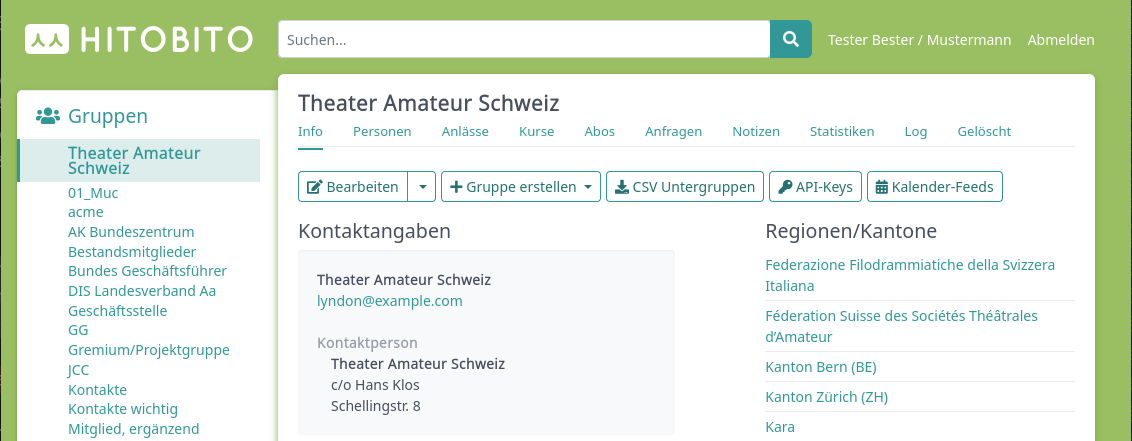
\includegraphics[width=1\textwidth,]{group_overview.png}}
   \caption{Gruppenübersicht Hitobito}
\end{figure}

\newpage

Danach werden unter dem Reiter ``Personen'' alle Personen der ausgewählten Gruppe angezeigt.
\begin{figure}[h]
   \centering
   \fbox{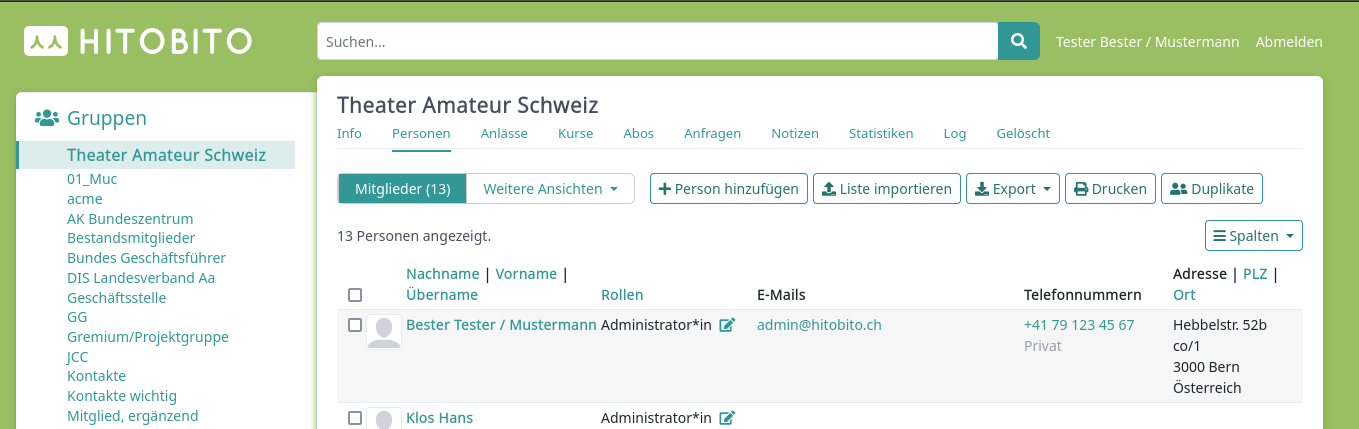
\includegraphics[width=1\textwidth,]{people_overview.png}}
   \caption{Personenübersicht Hitobito}
\end{figure}

Unter dem Dropdown ``Weitere Ansichten'' kann der User entweder einen bestehenden Personenfilter auf die angezeigte Personenliste anwenden 
oder einen neuen Personenfilter erstellen. Der neue Personenfilter kann unter der Option ``Neuer Filter...'' erstellt werden.

\begin{figure}[h]
   \centering
   \fbox{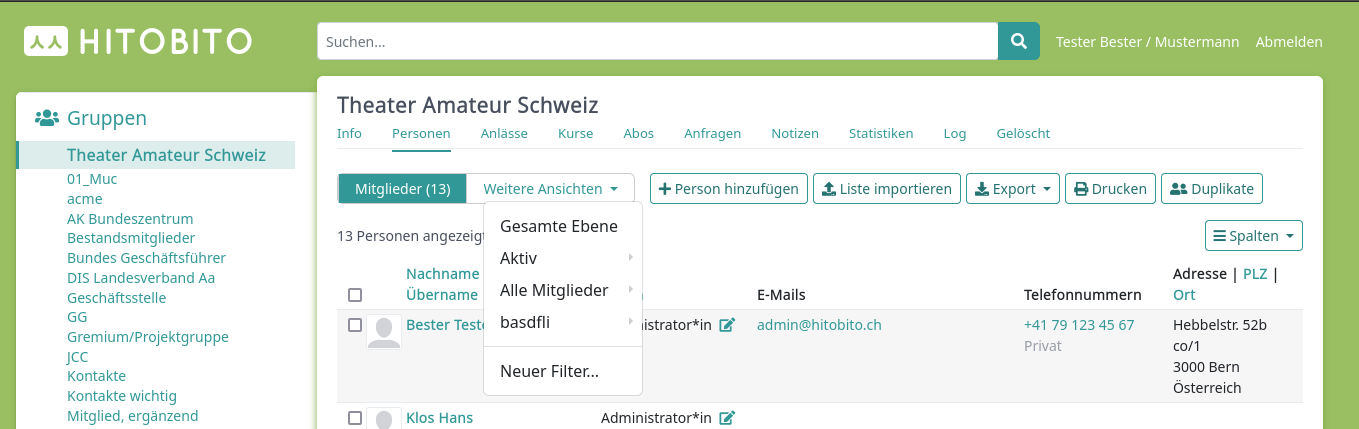
\includegraphics[width=1\textwidth,]{filter_selection.png}}
   \caption{Filterauswahl Hitobito}
\end{figure}

\newpage

Nach dem Klick auf diese Option wird der Benutzer auf eine Filterübersicht weitergeleitet. Die Filterübersicht besteht aus Buttons für die Speicher und Suche, drei Radio-Buttons und fünf Dropdowns.

Die drei Radio-Buttons zu Beginn definieren auf welcher Ebene gesucht wird.
Jedes Dropdown bietet dem Benutzer die Möglichkeit Filterkriterien zu definieren. Die Art des Filterkriteriums ist durch
den Dropdownnamen gegeben.


\begin{figure}[h]
   \centering
   \fbox{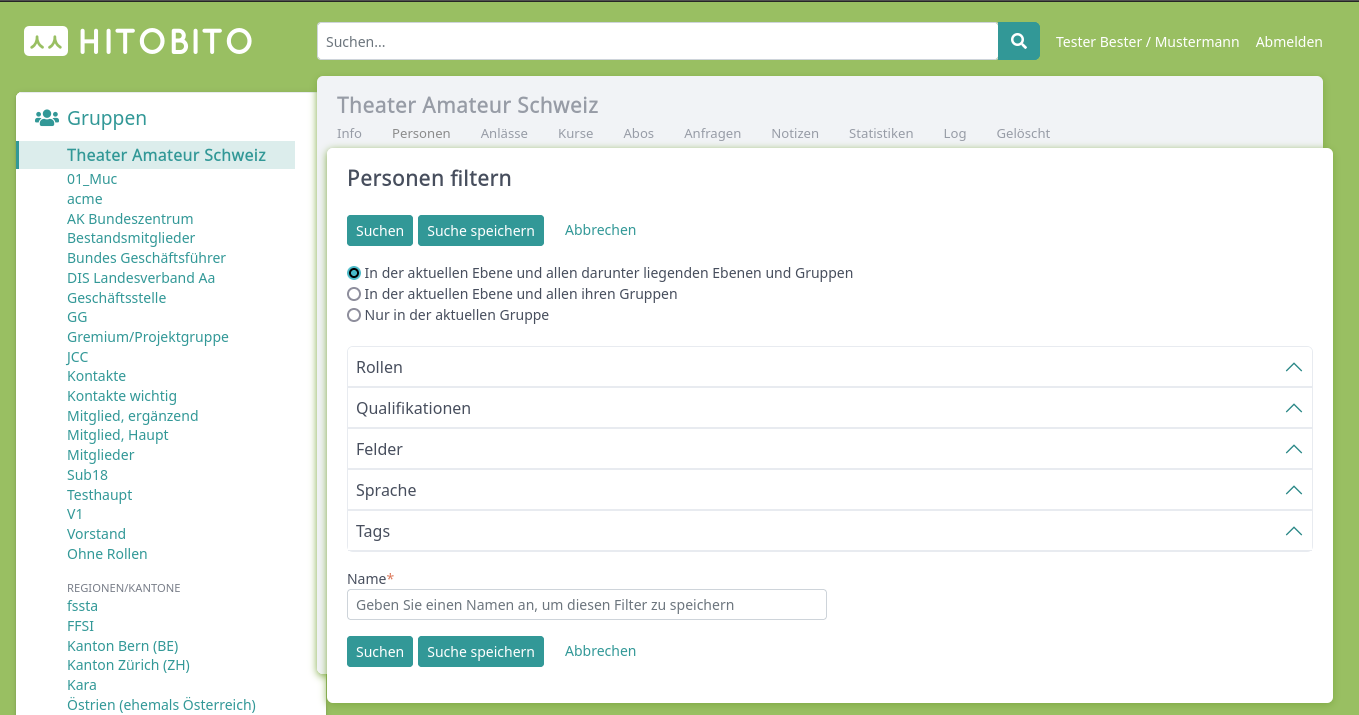
\includegraphics[width=1\textwidth,]{filter_overview.png}}
   \caption{Filterübersicht Hitobito}
\end{figure}

\newpage

Im Dropdown ``Rollen'' werden alle Rollen pro Ebene aufgelistet. Der Benutzer kann per Klick auf eine Checkbox
die Rollen auswählen, welche Personen durch die Filterung aufweisen müssen. Möchte der Benutzer alle Rollen einer Ebene auswählen,
kann er die mit einem Klick auf den Namen einer Ebene tun. In diesem Beispiel wäre das ein Klick auf ``Hauptebene''. Nach dem Klick auf den
Ebenennamen werden alle Checkboxen abgehakt. Somit wurden alle Rollen der angeklickten Eben ausgewählt.

Für die Rollen kann des weiteren ein Gültigkeits-Zeitraum definiert werden. Die Gültigkeit
wird vom Benutzer via Radio-Buttons ausgewählt. Zuletzt kann im ``Rollen'' Dropdown entschieden werden, ob 
archivierte Rollen bei der Filterung berücksichtigt werden. Das UI bietet dem Benutzer dafür eine weiter selbststehende
Checkbox.

\begin{figure}[h]
   \centering
   \fbox{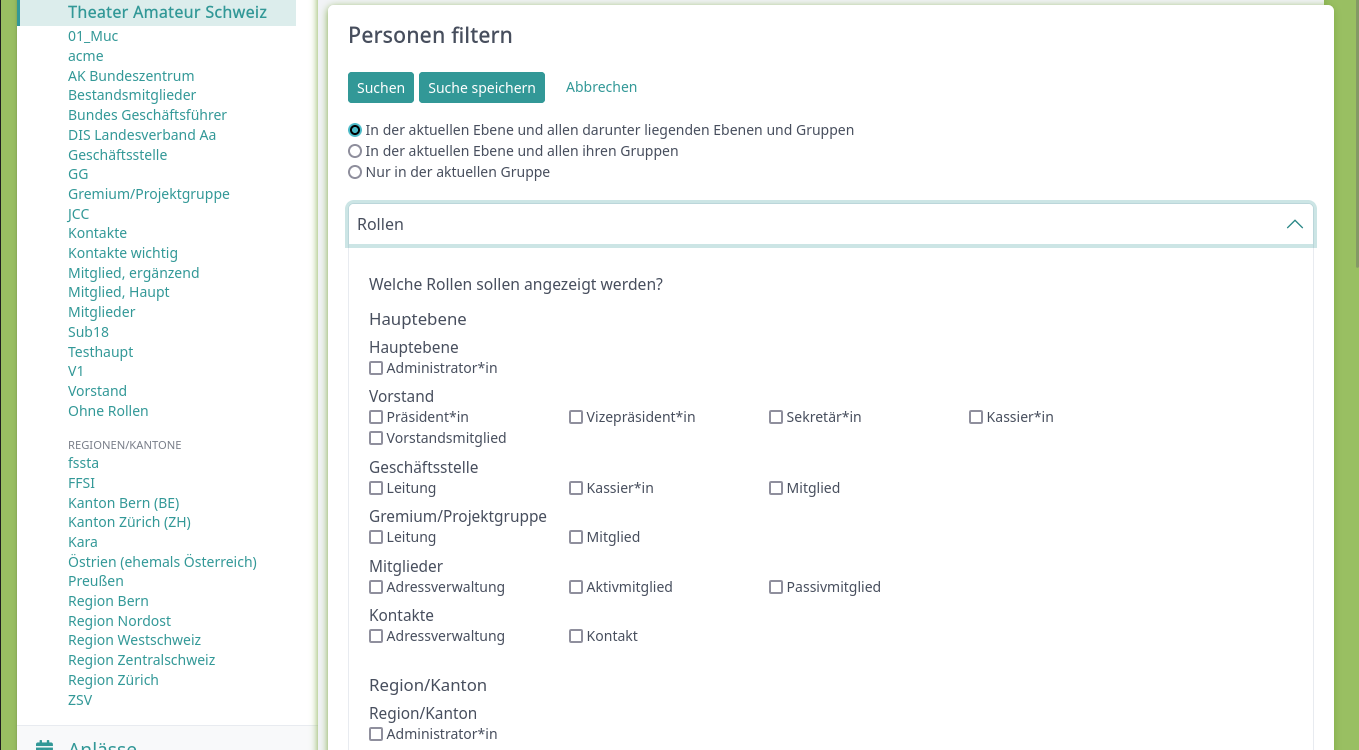
\includegraphics[width=1\textwidth,]{role_overview.png}}
   \caption{Filterkriterium Rollen}
\end{figure}

\begin{figure}[h]
   \centering
   \fbox{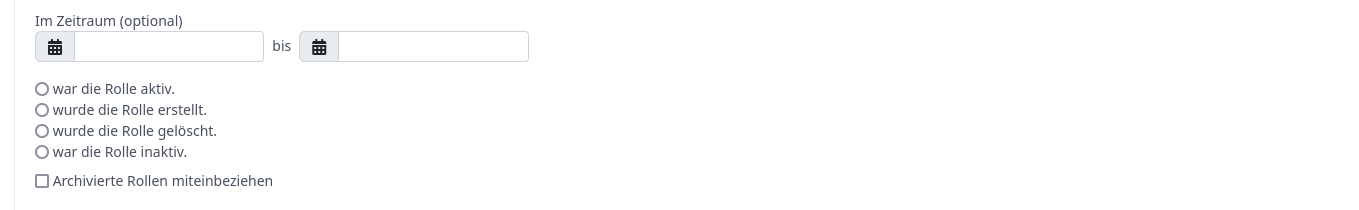
\includegraphics[width=1\textwidth,]{additional_role_options.png}}
   \caption{Filterkriterium Rollen - Zeitraum und Archivierung}
\end{figure}

\newpage

Im Dropdown ``Qualifikationen'' werden alle auswählbaren Qualifikationen angezeigt.
Der Benutzer wählt alle gewünschten Qualifikationen per Checkbox aus. Per Radio-Button entscheidet
der Benutzer danach, ob die Person alle oder mindestens eine der angeklickten Rollen aufweisen muss.

Abschliessen für die Qualifikationen kann die Gültigkeit per Radio-Buttons und ein Stichdatum
per Input-Feld definiert werden.

\begin{figure}[h]
   \centering
   \fbox{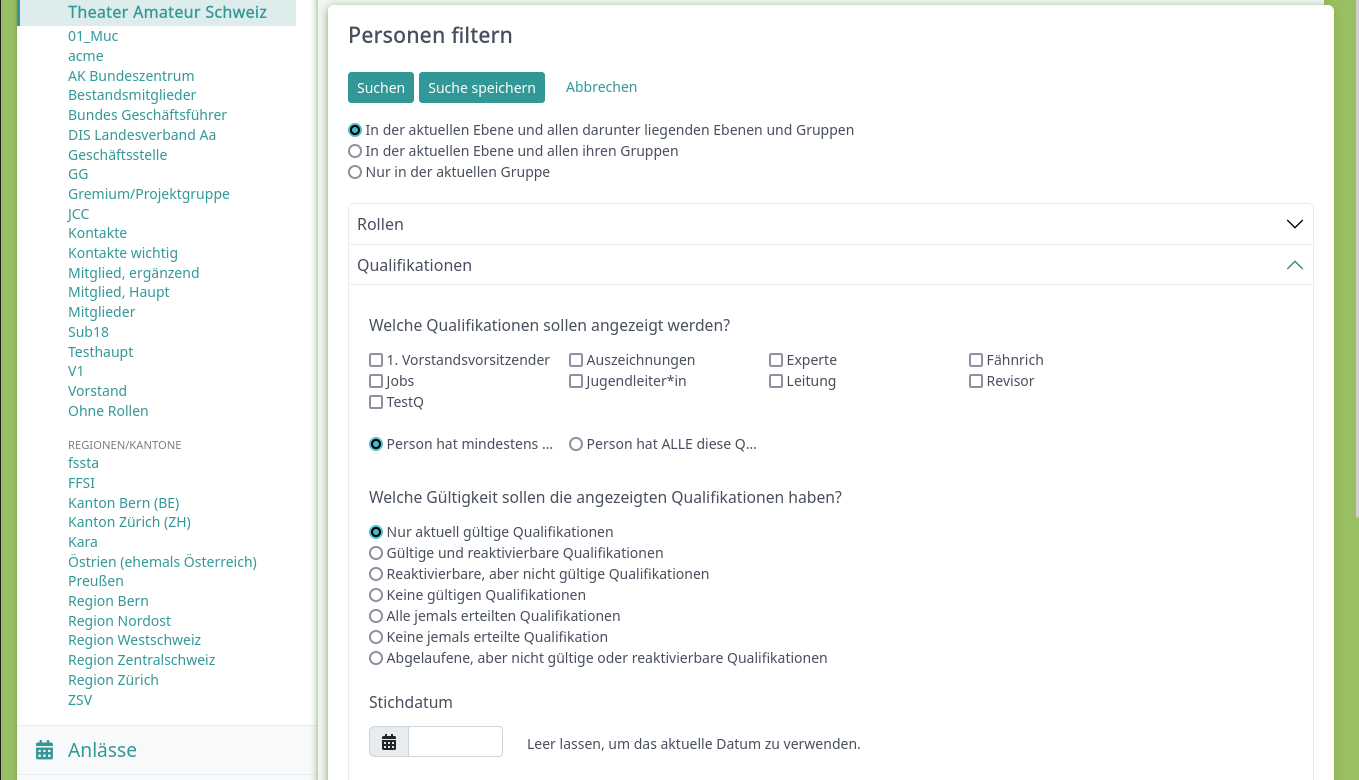
\includegraphics[width=1\textwidth,]{qualification_overview.png}}
   \caption{Filterkriterium Qualifikationen}
\end{figure}

Beim Filterkriterium ``Felder'' handelt es sich um zusätzliche Personenattribute welche in
die Filterung miteinbezogen werden.

\begin{figure}[h]
   \centering
   \fbox{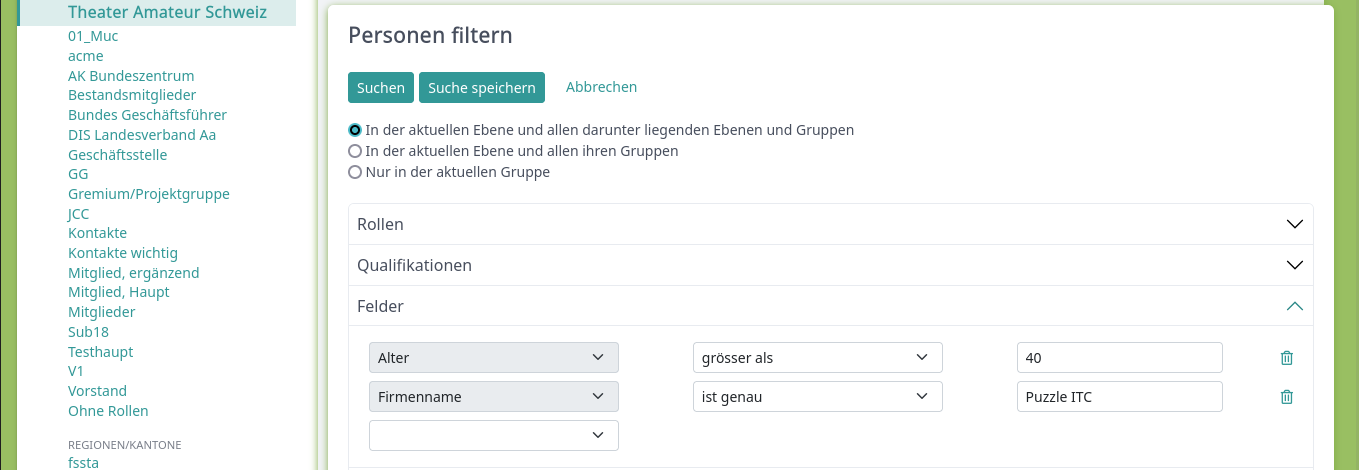
\includegraphics[width=1\textwidth,]{field_overview.png}}
   \caption{Filterkriterium Felder}
\end{figure}

\newpage

Unter die Kategorie der ``Felder'' fallen folgende Personenattribute:

\begin{table}[h!]
   \begin{tabular}{|L{0.5\textwidth}|L{0.5\textwidth}|}
       \hline
       \rowcolor{puzzleblue}\color{white}Attribut & \color{white}Datentyp \\
       \hline
       Alter & Zahl \\
       \hline
       Firmenname & Text \\
       \hline
       Geburtstag & Zeit \\
       \hline
       Geschlecht & Text \\
       \hline
       Haupt-E-Mail & Text \\
       \hline
       Hausnummer & Zahl \\
       \hline
       Land & Text \\
       \hline
       Nachname & Text \\
       \hline
       Ort & Text \\
       \hline
       PLZ & Zahl \\
       \hline
       Postfach & Text \\
       \hline
       Strasse & Textwert \\
       \hline
       Vornamen & Textwert \\
       \hline
       Zusätzliche Adresszeile & Textwert \\
       \hline
       Übername & Textwert \\
       \hline
     \end{tabular}
     \caption{Felder-Attribute}
\end{table}

Die Attribute können über ein Dropdown ausgewählt werden. Wurde das Attribut ausgewählt kann zusätzlich die Genauigkeit
des Filterkriterums definiert werden.

Für Textwerte bieten sich folgende Genauigkeiten an:

\begin{itemize}
   \item ist genau
   \item enthält
   \item enthält nicht
\end{itemize}

Für Zahlenwerte bieten sich folgende Genauigkeiten an:

\begin{itemize}
   \item ist genau
   \item ist grösser als
   \item ist kleiner als
\end{itemize}

So kann der Benutzer bestimmen wie genau sein eingegebener Wert dem ausgewählten Attribut entsprechen soll.

\newpage

Das Filterkriterium ``Sprachen'' bietet die Möglichkeit aus den Optionen Deutsch, Englisch oder Französisch auszuwählen.
Es können auch mehrer Sprachen ausgewählt werden. Die Auswahl erfolgt über Checkboxen.

\begin{figure}[h]
   \centering
   \fbox{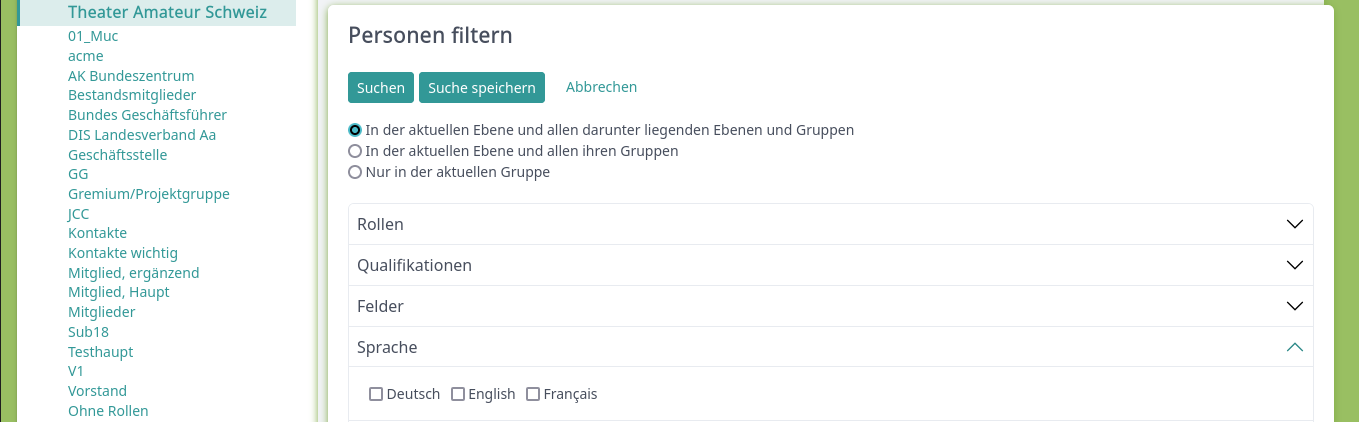
\includegraphics[width=1\textwidth,]{language_overview.png}}
   \caption{Filterkriterium Sprache}
\end{figure}


Das Filterkriterium ``Tags'' macht es möglich Personen nach gegebenen Tags zu suchen. Über zwei 
Inputfelder kann definiert werden, welche Tags eine Person haben oder nicht haben muss. Die Input-Felder sind
Dropdowns welche dem Benutzer die Eingabe vervollständigen wenn dieser nach einem Tag sucht.

\begin{figure}[h]
   \centering
   \fbox{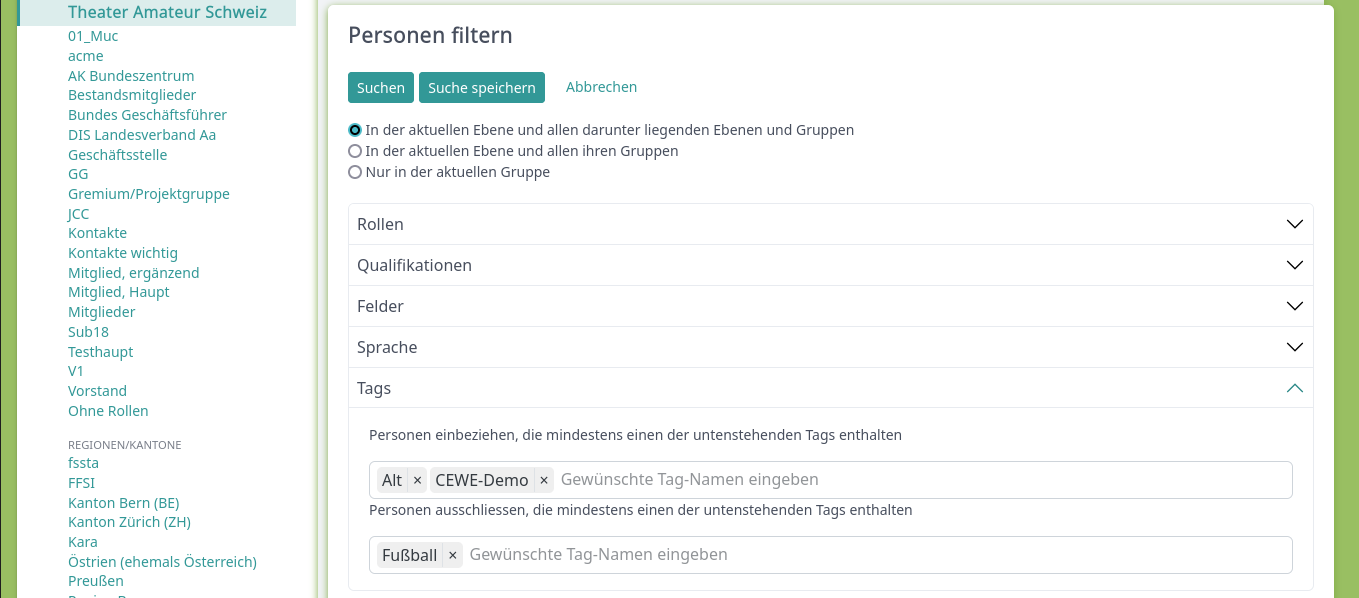
\includegraphics[width=1\textwidth,]{tag_overview.png}}
   \caption{Filterkriterium Tags}
\end{figure}

\newpage

Wurden alle Filterkriterien vom Benutzer definiert kann dieser die Konfiguration des Personenfilters speichern. 
Dazu muss ein Name des Filters definiert werden. Will der Benutzer den Filter nicht speichern, kann der auf den Button ``Suchen'' klicken. Anschliessend
werden auf der Personenübersicht nur Personen angezeigt welche die Filterkriterien erfüllen. Wird der Filter nicht gespeichert, 
muss dieser erneut von Hand zusammengestellt werden.

\begin{figure}[h]
   \centering
   \fbox{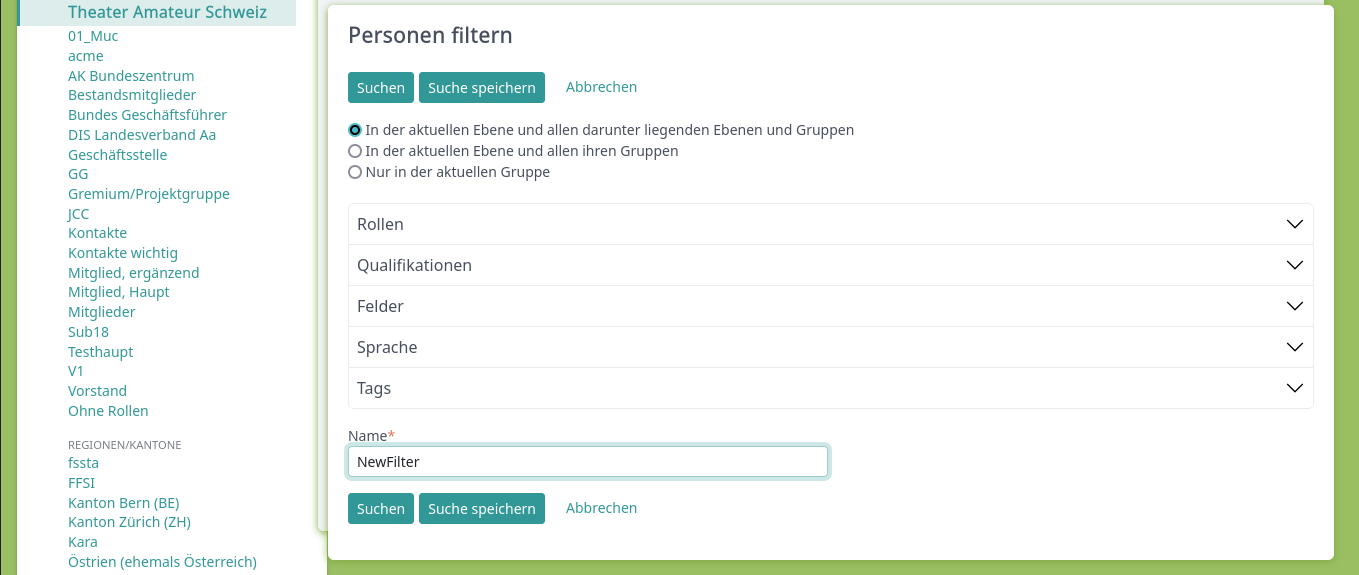
\includegraphics[width=1\textwidth,]{saving_filter.png}}
   \caption{Filterkriterium Tags}
\end{figure}

\newpage

\subsection{Abonnemente}
Die Abonnementenfilterung kann nicht im Hitobito wie die Personenfilterung angezeigt werden. Stattdessen
wird die Filterung bei einem Export von Abonnementen als CSV angewendet. So werden im resultierenden CSV nur Personen
angezeigt, welche den Filterkriterien entsprechen.

Die Abonnementenfilterung kann erneut über die Gruppenübersicht ausgemacht werden.

\begin{figure}[h]
   \centering
   \fbox{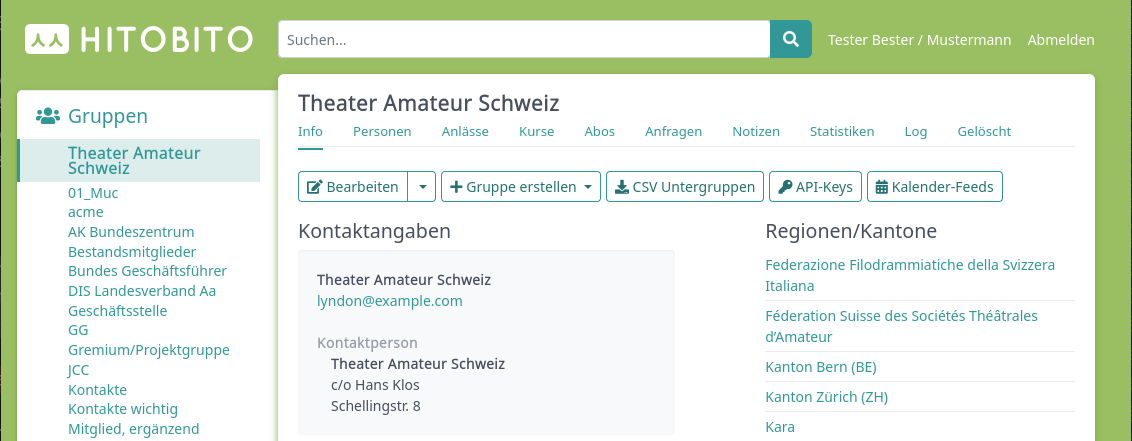
\includegraphics[width=1\textwidth,]{group_overview.png}}
   \caption{Gruppenübersicht}
\end{figure}

Danach muss auf den Reiter ``Abos'' navigiert werden.

\begin{figure}[h]
   \centering
   \fbox{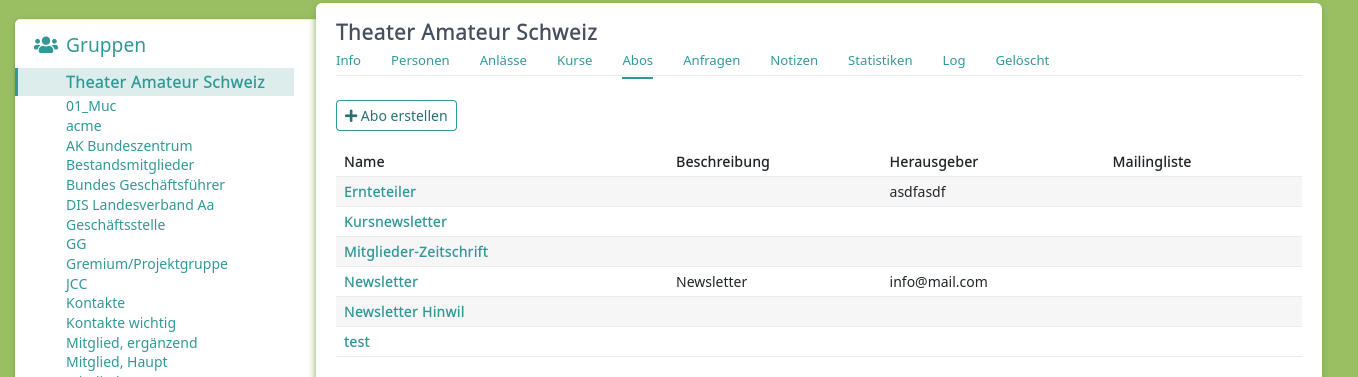
\includegraphics[width=1\textwidth,]{subscription_overview.png}}
   \caption{Abonnementen Übersicht}
\end{figure}

Auf dieser Ansicht kann der Benutzer per Klick ein Abonnement auswählen.

\newpage

Daraufhin wird der Benutzer auf die Infoseite des Abonnements weitergeleitet. Um die Abonnementenfilterung
einzusehen muss nun auf den Reiter ``Abonnementen'' navigiert werden.

\begin{figure}[h]
   \centering
   \fbox{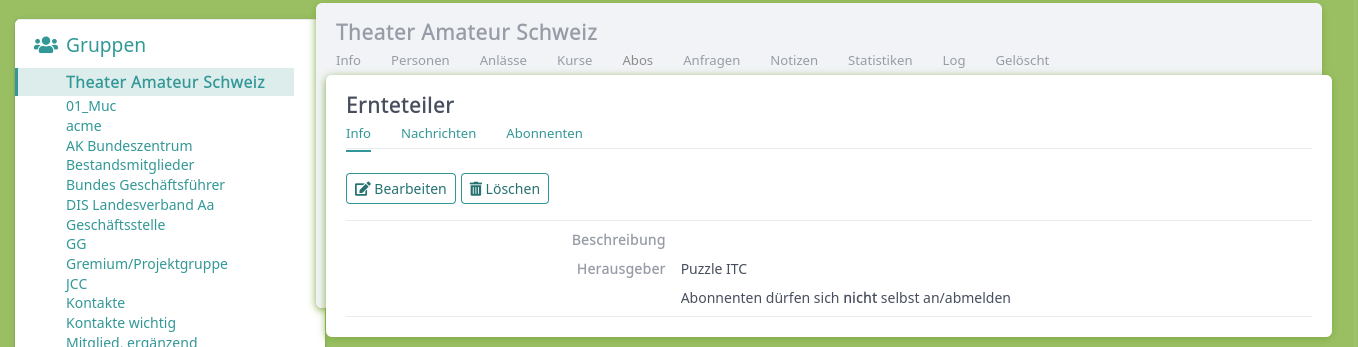
\includegraphics[width=1\textwidth,]{single_subscription_overview.png}}
   \caption{Übersicht einzelnes Abonnement}
\end{figure}

Unter dieser Ansicht ist es dem Benutzer möglich diverse Filterkriterien für das Abonnement zu definieren.
Im Rahmen dieser IPA werden ausschliesslich die globalen Bedingungen überarbeitet, weswegen die anderen Filterkriterien
zu vernachlässigen sind. Die globalen Bedingungen können über das Bearbeitungssymbol angepasst werden.

\begin{figure}[h]
   \centering
   \fbox{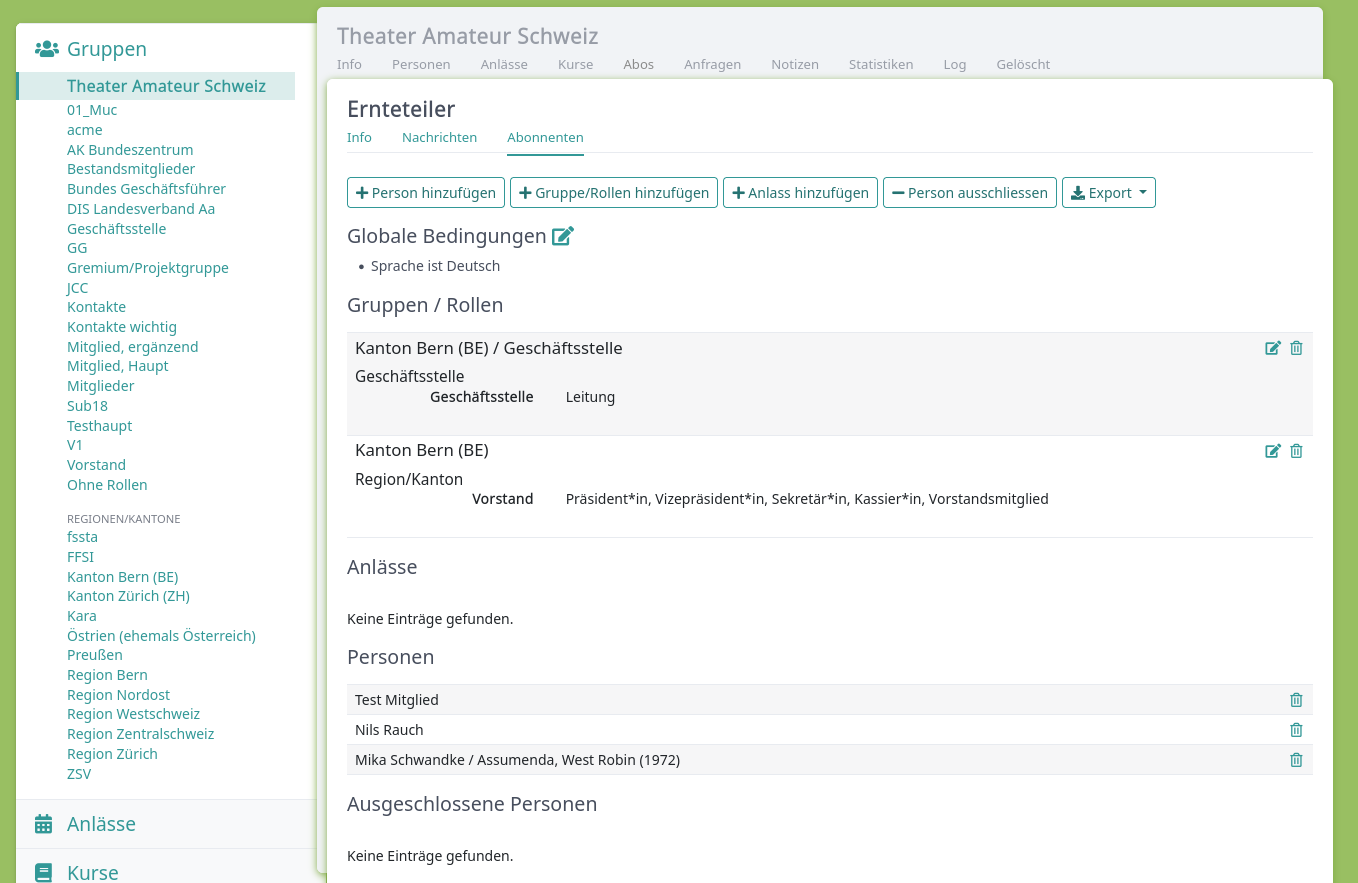
\includegraphics[width=1\textwidth,]{subscription_filter_overview.png}}
   \caption{Abonnementenübersicht}
\end{figure}

\newpage


In den globalen Bedingungen bieten sich zwei Filterkriterien: Felder und Sprache. Die Funktionsweise
ist dabei die gleiche, wie die der Personenfilter (weiter oben beschrieben).

Der Benutzer wählt die Filterkriterien aus und Speichert diese anschliessend. Die gespeicherten Bedingungen 
werden in der Textbox unter dem Titel ``Globale Bedingungen'' auf der Abonnementenübersicht angezeigt.
\begin{figure}[h]
   \centering
   \fbox{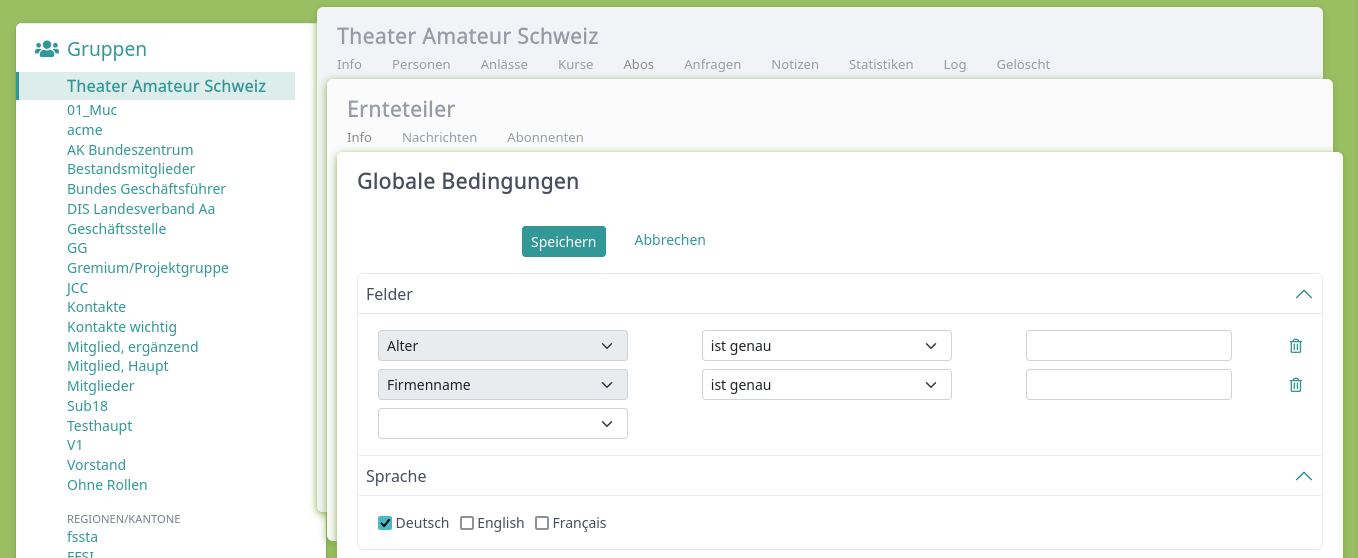
\includegraphics[width=1\textwidth,]{global_conditions_overview.png}}
   \caption{Globale Filterungsbedingungen für Abonnemente}
\end{figure}

\newpage

\section{Soll-Zustand}
In der Vorarbeit für diese IPA wurde vom Kandidaten ein Mockup erstellt. Das Produkt der IPA soll nach diesem Mockup umgesetzt werden.
Das angefertigte Mockup repräsentiert den Soll-Zustand und wird im folgenden Abschnitt erklärt.

\subsection{Anzeigemasken}
Zuerst werden die Anzeigemasken des Mockups vorgestellt. Dabei handelt es sich um Anzeigen, welche der Benutzer ausschliesslich lesen und nicht
bearbeiten kann.

\textbf{Filterübersicht}
Sobald der Benutzer auf ``Neuer Filter...'' in der Personenübersicht einer Gruppe klickt, soll er auf folgende Ansicht weitergeleitet werden:

\begin{figure}[h]
   \centering
   \fbox{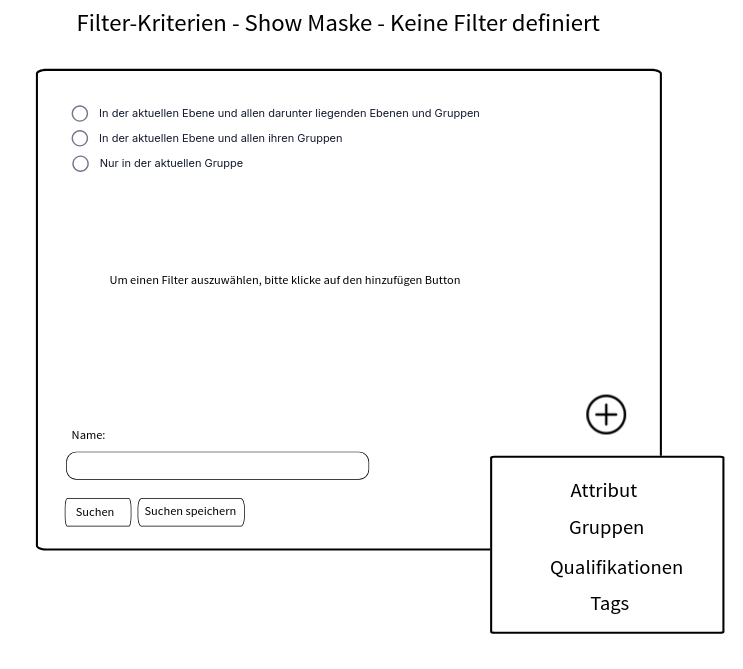
\includegraphics[width=0.8\textwidth,]{mockup_nofilter_overview.png}}
   \caption{Mockup Filterübersicht}
\end{figure}

Die Übersicht enthält die Radio-Buttons der alten Benutzerschnittstelle. Die massgäbliche Änderung zum Soll-Zustand betrifft den hinzufügen Button.
Dieser befindet agiert als Dropdown, sobald der Benutzer auf ihn klickt. Das Dropdown besitzt vier Filterungskriterien, nicht mehr die fünf wie sie momentan
im Hitobito anzutreffen sind. Sind noch keine Filterkriterien erfasst, wird dies dem Benutzer mit einem Text signalisiert.
Die Speicherungskomponente des Filters bleibt bestehen.

\textbf{Filterübersicht mit Tags und Felder}

Hat der Benutzer seine Filterkriterien definiert, werden diese in Boxen angezeigt.
Die definierte Filterkriterien verschwinden aus dem Dropdown unter dem Hinzufüge-Butto. Stattdessen können 
die definierten Filterkriterien über den Stif in der oberen, rechten Ecke einer Box bearbeitete werden.

\begin{figure}[h]
   \centering
   \fbox{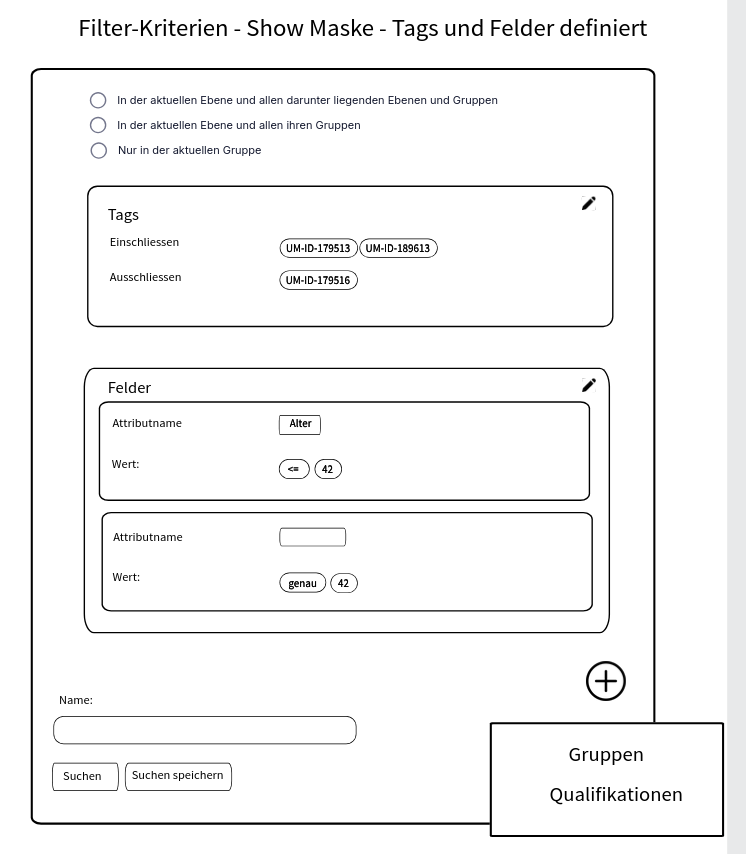
\includegraphics[width=0.8\textwidth,]{mockup_two_filters.png}}
   \caption{Mockup mit Tags und Felder definiert}
\end{figure}

In dieser Ansicht hat der Benutzer das Filterkriterium ``Tags'' und ``Felder'' definiert. Diese Optionen verschwinden
somit aus dem Dropdown. Wurden zu jedem Filterkriterium Bedingungen erfasst, verschwindet der gesamte Hinzufüge-Button.

\newpage

\textbf{Filterübersicht mit Qualifikationen und Rollen}

Im folgenden Bild hat der Benutzer Tags, Rollen und Qualifikationen als Filterkriterien erfasst.

\begin{figure}[h]
   \centering
   \fbox{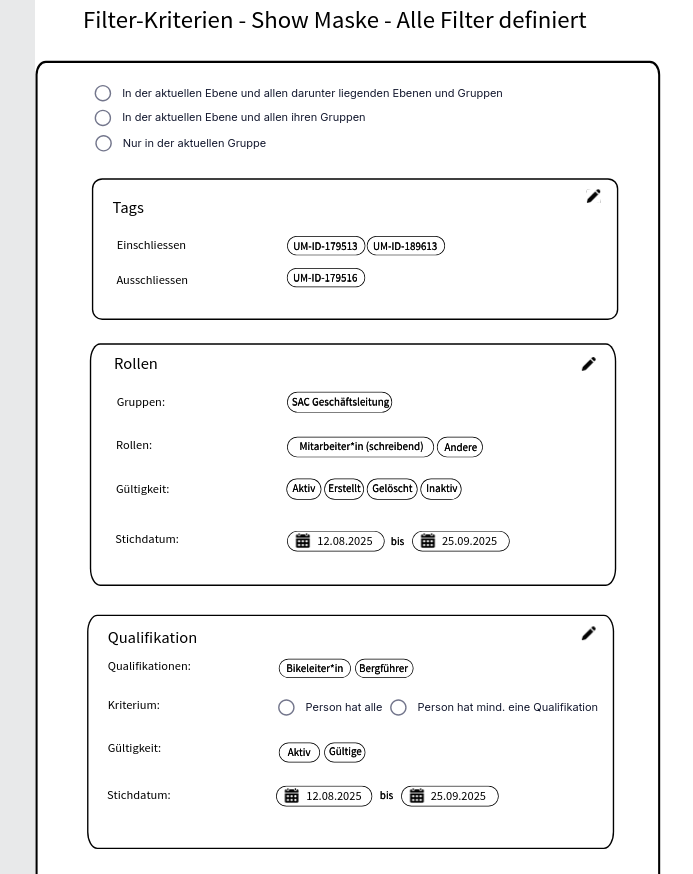
\includegraphics[width=0.8\textwidth,]{mockup_roles_qualifications.png}}
   \caption{Mockup mit Qualifikationen und Rollen definiert}
\end{figure}

\subsection{Bearbeitungsmasken}
Nachfolgend werden die Anzeigen vorgestellt, welche der Benutzer bearbeiten kann. Diese sind für den Benutzer zugänglich, indem er
ein Filterkriterium entweder per Hinzufüge-Button hinzufügt oder per Editier-Button (Stift in der oberen rechten Ecke der Box) bearbeitet.

\textbf{Felder}

Die Felder können im neuen Mockup durch ein Dropdown ausgewählt werden. Danach wird kann wie zuvor die Genauigkeit bestimmen werden.
Will der Benutzer ein weiteres Attribut zu seinen Suchbedingungen hinzufügen, kann er dies über den Hinzufüge-Butten in der rechten unteren Ecke. Auf dieser
Benutzerschnittstelle ist es möglich die Sprache als Attribut auszuwählen. Für die Sprache kann standardmässig keine Genauigkeit definiert werden.

\begin{figure}[h]
   \centering
   \fbox{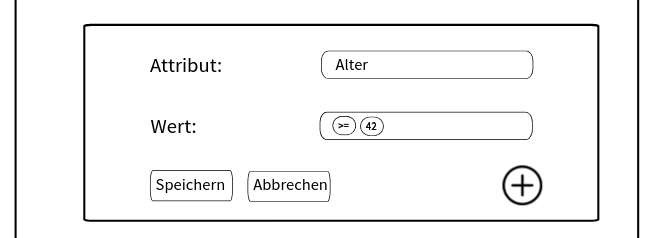
\includegraphics[width=0.8\textwidth,]{mockup_attributes.png}}
   \caption{Bearbeitungsmaske Filterkriterium Felder}
\end{figure}

\newpage

\textbf{Rollen}

Die Rolle kann über die Gruppe oder den Rollennamen definiert werden. Wird unter dem Eingabefeld ``Gruppen'' eine Gruppe hinterlegt,
werden alle dazugehörigen Rollen dieser Gruppe in die Filterung miteinbezogen. Will der User nur einzelne Rollen
in die Filterung miteinbeziehen, kann er dies über das Rollen-Eingabefeld. Die Gültigkeit der Rolle wird kann über ein suchbares dropdown ausgewählt werden.
Das Element der Stichdatum bleibt bestehen. Die Checkbox für die archivierten Rollen wird im Mockup vernachlässigt und standardmässig werden alle Rollen,
sofern diese die Gültigkeitsbedingungen erfüllen, miteinbezogen.

\begin{figure}[h]
   \centering
   \fbox{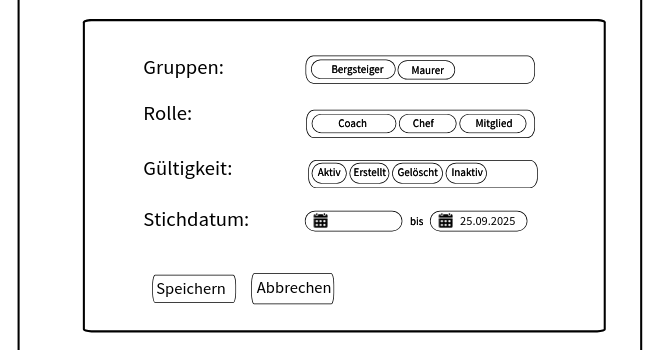
\includegraphics[width=0.8\textwidth,]{mockup_roles.png}}
   \caption{Bearbeitungsmaske Filterkriterium Gruppe}
\end{figure}

\newpage

\textbf{Qualifikationen}

Die Qualifikationen können innerhalb der Bearbeitungsmaske ebenfalls mit einem suchbaren Dropdown 
ausgewählt werden. Die Radio-Buttons und das Stichdatum bestehen wie bisher. Die Gültigkeit kann wie bei den Rollen über 
ein suchbares Stichdatum ausgewählt werden.

\begin{figure}[h]
   \centering
   \fbox{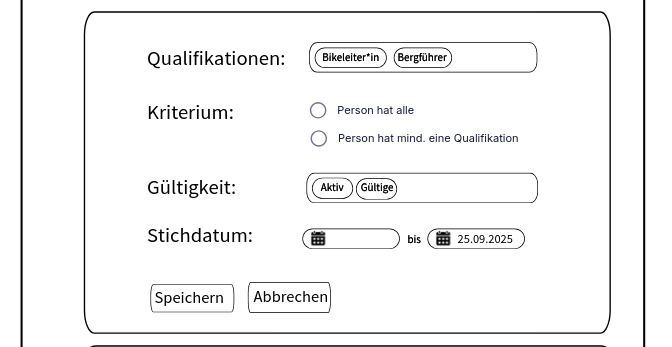
\includegraphics[width=0.8\textwidth,]{mockup_qualifications.png}}
   \caption{Bearbeitungsmaske Filterkriterium Qualifikationen}
\end{figure}

\textbf{Tags}

Die Definition der Tags bleibt bestehen wie in der Soll-Situation beschrieben

\begin{figure}[h]
   \centering
   \fbox{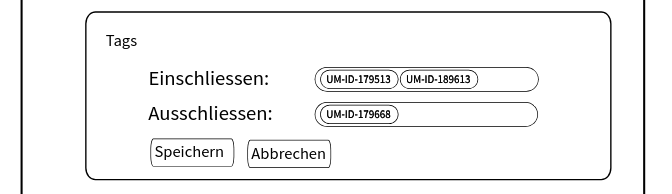
\includegraphics[width=0.8\textwidth,]{mockup_tags.png}}
   \caption{Bearbeitungsmaske Filterkriterium Tags}
\end{figure}

\newpage

\section{Fehlende Informationen}
Alle bekannten Informationen bei Beginn der IPA wurden in der Ist-Situation und der Soll-Situation beschrieben.
Als unbekannte Informationen gelten: Die Bedürfnisse des Benutzers, Sicherheitsrisiken, sowie die darauf resultierenden Produktanforderungen.
Die genannten Bereiche werden in den kommenden Abschniten aufgenommen und analysiert. Alle unbekannten Informationen welche einzelne 
Definitionen oder Abläufe betreffen wurden über das Internet oder KI recherchiert und anschliessend im Anhang unter dem Datum der Verwendung hinterlegt.

\newpage

\section{Bedürfniserhebung}
Um die Bedürfnisse der Kunden vor der Entwicklung zu identifizieren wird eine Bedürfniserhebung durchgeführt. 
Angewendete Modelle, Befragungstechniken und Erhebungen werden im folgenden Abschnitt dokumentiert. Es wird zuerst die Zielsetzung und Planung definiert,
danach die Methode der Erhebung ausgewählt, die Erhebung durchgeführt und zuletzt alle Daten und identifizierten Bedürfnisse analyisert.

\subsection{Zielsetzung und Planung}
Mit dieser Bedürfnisserhebung sollen Anforderungen an das Produkt auf Kundenseite ausgemacht werden. Aus zeitlichen Gründen
werden die Anforderung einer Person an das Produkt analysiert. Bei der Person handelt es sich um Thomas Ellenberg, dem Projektleiter von Hitobito.
Für die Bedürfniserhebung wurden vier Stunden geplant. Zwei Stunden werden für die Vorbereitung verwendet, eine Stunde für die Durchführung und
eine Stunde für die Auswertung der Erhebung. 

Beteiligt an der Bedürfniserhebung sind Marc Egli und Thomas Ellenberg. Marc Egli ist für die
Durchführung der Erhebung zuständig. Da die Bedürfniserhebung im Rahmen der IPA durchgeführt wird, wird mit keinem Budget geplant.

\subsection{Methodenwahl}

Es stehen vier Methoden zur Bedürfniserhebung zur Verfügung:

\begin{itemize}
   \item Umfragen
   \item Interviews und Fokusgruppen
   \item Beobachtungen
   \item Dokumentenanalyse
\end{itemize}

\newpage

In dieser Arbeit wurde als Methode das Interview gewählt. Die Begründung resultiert aus folgendem Ausschlussverfahren:

\begin{table}[h!]
   \begin{tabular}{|L{0.2\textwidth}|L{0.5\textwidth}|L{0.2\textwidth}|}
       \hline
       \rowcolor{puzzleblue}\color{white}Methode & \color{white} Gedankengänge & \color{white} Verwendung \\
       \hline
       Umfragen & Hiefür wird eine grosse Benutzergruppe benötigt um ein aussagekräftiges Resultat daraus zu ziehen. 
       Für die Organisation einer solchen Benutzergruppe besteht keine Zeit. & Nein \\
       \hline
       Interviews und Fokusgruppen & Durch ein Interview können mehr Informationen gewonnen werden als einer Umfrage.
       Bspw. Beobachtungen der Gefühle des Benutzers oder Gedankengänge können aufgenommen werden. Um dennoch den Zeitrahmen der IPA
       nicht zu verletzen, müsste das Inteview mit nur einer Person durchgeführt werden. & Ja \\
       \hline
       Beobachtungen & Um Bedürfnisse mit einer Beobachtung durchzuführen, muss zuerst ein Testskript geschrieben werden.
       In einem Testskript muss jeder Schritt und die daraus folgenden Aufgabe klar definiert sein. Dies gelöscht
       mit einem hohen Zeitaufwand für die Verfassung des Testskripts einher. & Nein \\
       \hline
       Dokumentenanalyse & Die Dokumentenanalyse kann mit dem Benutzerhandbuch von Hitobito durchgeführt werden.
      Die daraus entstehenden Bedürfnisse würden aber vom Analyst selbst kommen, nicht direkt vom Benutzer. & Nein \\
     \hline
     \end{tabular}
     \caption{Methodenwahl}
\end{table}

\newpage

\subsection{Fragenkatalog}
Die Fragen im Interview basieren auf dieser \href{https://kreativ.mfg.de/digitale-kultur/kompass-digitale-kultur/prozess/nutzerinnen-gruppe/bedarfsanalyse-interviews/}{Anleitung}.
Während des Interviews werden die nachkommenden Fragen gestellt:

\textbf{Offene Einleitungsfragen}
\begin{itemize}
   \item Frage 1: Was bist du für eine Person? Beschreibe dich kurz
   \item Frage 2: Was ist dir wichtig im Leben?
   \item Frage 3: Welchen Karriereweg hast du hinter dir? 
   \item Frage 4: Wie kamst du das erste Mal in Kontakt mit Hitobito?
\end{itemize}

\textbf{Fragen zu Hitobtio allgemein}
\begin{itemize}
   \item Frage 5: Was fasziniert dich an Hitobito?
   \item Frage 6: Welche Teile der Applikation stören dich selbst?
\end{itemize}

\textbf{Fragen zur Hitobito Filterung}
\begin{itemize}
   \item Frage 7: Welche Erfahrungen hast du mit der Filterung von Personen und Abonnemente in Hitobito gemacht?
   \item Frage 8: Was stört dich an dieser Filterung?
   \item Frage 9: Was würdest du an dieser ändern Filterung?
   \item Frage 10: Welche zusätzlichen Funktionen wünschst du dir für diese Filterung?
   \item Frage 11: Wie würdest du alle Mängel und zusätzlichen Features auf priorisieren?
   \item Frage 12: Welchen Dringlichkeit hat eine Überarbeitung der Filterung für dich?
   \item Frage 13: Welche Kosten wärst du maximal bereit zu zahlen?
\end{itemize}

\newpage

\subsection{Ablaufsprotokoll}
\begin{table}[h!]
   \begin{tabular}{|L{0.2\textwidth}|L{0.4\textwidth}|L{0.3\textwidth}|}
       \hline
       \rowcolor{puzzleblue}\color{white}Tätigkeit & \color{white} Antwort der Testperson & \color{white} Mimik und Gestik \\
       \hline
       Begrüssung der Testperson & Danke vielmals für die Einladung. & Testperson scheint positiv eingestimmt zu sein, ein bisschen nervös. \\
       \hline
       Erklärung des Ablaufs & Perfekt, ja das stimmt so für mich. & Testperson richtet Blick aufmerksam auf den Befrager. \\
       \hline
       Frage 1 & Ich bin Product Owner von Hitobito teilweise. Eigentlich ist Oliver Dietschi der Product Owner, aber ich höre von vielen Kunden was ihre Bedürfnisse sind. & Testperson Lächelt leicht. \\
       \hline
       Frage 2 & Im Moment ist mir Nachhaltigkeit unheimlich wichtig. Bei allen Bereichen, Beziehungen und Freundschaften. Auch was ich kaufe und wie ich leben. & Testperson wird ernster. Stimme senkt sich. \\
       \hline
       Frage 3 & Ich habe ursprünglich das KV beim Inter Discount gemacht. Im Detailhandel. Danach habe ich bei der Swisscom gearbeiten und später gemerkt, dass das wohl doch nichts für mich ist. Danach habe ich ein
       Wirtschaftsstudium an der BFH gemacht. Dort habe ich gemerkt das mir Projektmanagement sehr zusagt. Anschliessend habe ich im Bereich Ausbildung und in der Stahlindustrie gearbeitet, dort als Projektmanager.
       Schlussendlich bin ich in der IT gelandet. & Testperson ist ernster zu Beginn der Antwort, lächelt beim Übergang zu der IT.   \\
       \hline
     \end{tabular}
     \caption{Ablaufsprotokoll Teil 1}
\end{table}

\newpage

\begin{table}[h!]
   \begin{tabular}{|L{0.3\textwidth}|L{0.4\textwidth}|L{0.2\textwidth}|}
       \hline
       \rowcolor{puzzleblue}\color{white}Tätigkeit & \color{white} Antwort der Testperson & \color{white} Mimik und Gestik \\
       \hline
       Frage 4 & Ich war selber ein sehr engagierter Pfadiler. Ich wusste noch gar nicht wie Hitobito funktioniert. Ein Kollege von mir, Tobi Hinderling, hatte
       dann von einer Firma namens Puzzle ITC gehört welche Hitobito betreibt. Er sagt sie sein super cool organisiert und er wolle unbedingt dort arbeiten. Das machte er
       dann auch und hatte das Projektmanagement bei Hitobito inne. Tobias und ich, wir waren immer wieder am Aareböttle zusammen und da hat er mir gesagt ich soll doch auch zu Puzzle kommen,
       denn ihn würde mer das UX als das Projektmanagement interessiern. Wir könnten dann intern die Rollen wechseln und genau so ist es geschehen. & Testperson Lacht bei der Anektote zu Tobias Hinderling. \\
       \hline
       Frage 5 & Die Kunden faszinieren mich an Hitobito. Wir haben eine sehr breite Kundenpalette. Wir streben auch eine langfristige Kunden an und nehmen nicht jeden.
       Wir haben sehr viele Non-Profit Gruppen und generell auch sehr angenehme Kunden. & Denkt kurz nach, ist ernster bei der Antwort. \\
       \hline
       Frage 6 & Das war sehr lange her. Keine Ahnung. Zu lange her. & Schüttelt Kopf. \\
       \hline
       Frage 7 & Ich habe die Filterung auch schon verwendet aber meist im Umfang von Tests und Abnahme der Akzeptanzkriterien von Tickets. & Testperson nickt als Bestätigung. \\
     \hline
     \end{tabular}
     \caption{Ablaufsprotokoll Teil 2}
\end{table}

\newpage

\begin{table}[h!]
   \begin{tabular}{|L{0.3\textwidth}|L{0.4\textwidth}|L{0.2\textwidth}|}
       \hline
       \rowcolor{puzzleblue}\color{white}Tätigkeit & \color{white} Antwort der Testperson & \color{white} Mimik und Gestik \\
       \hline
       Frage 8 & Was mich am meisten stört ist das UI. Alles ist ein bisschen verzettelt. Du weist nicht genau wo du suchen musst. Niemand weiss genau
       was man suchen kann. Die Filter können unheimlich viel, aber du musst ein bisschen suchen. & Gestikuliert in Richtung Laptop, Stimme wird lauter. \\
       \hline
       Frage 9 & Ich würde versuchen, alles zu vereinheitlichen. Evtl. z.B. die Felder und Sprache zusammennehmen. Auch die Rollen
       haben eine coole Funktion bei der Anwahl der Hauptebene. Aber diese Funktion kennt einfach niemand. Das müsste irgendwo genauer erklärt werden.
       Funktional ist enorm viel drin. Aber sie hegen einen gewissen Pain. & Testperson wird ruhiger, überlegt, Stimme wird leiser. \\
       \hline
       Frage 10 & Gute Frage. Nein ich glaube nicht, für mich hat die Filterung alles was sie bringt. Aber fairerweise brauche ich die Filterung
       ein bisschen zu wenig. & Testperson überlegt, Kopf seitlich angelegt, Stimme wird leiser. \\
     \hline
     \end{tabular}
     \caption{Ablaufsprotokoll Teil 3}
\end{table}

\newpage

\begin{table}[h!]
   \begin{tabular}{|L{0.3\textwidth}|L{0.4\textwidth}|L{0.2\textwidth}|}
       \hline
       \rowcolor{puzzleblue}\color{white}Tätigkeit & \color{white} Antwort der Testperson & \color{white} Mimik und Gestik \\
       \hline
       Frage 11 & Als erstes das Sprachen Dropdown aus der Landschaft entfernen und unter Felder anordnen. Der nervt mich tatsächlich sehr. So, wieso haben wir für jedes
       Attribut ein Dropdown in den Feldern aber für die Sprachen hängt es hier einfach so herum? Ansonsten finden
       ich alles andere OK. Geschlecht ist etwas anderes was mich stört. Dort muss du wenn du ein Mann bist ``m'' eingeben und wenn du eine Frau bist ``w''. 
       Auch ``w''' wenn du die Sprache auf Französisch eingestellt hast. Und weist du was? Wenn du kein Geschlecht hast musst du das Feld leer lassen, dass weiss einfach
       niemand. & Testperson regt sich auf, Gestikuliert in Richtung Hitobito Filterung auf Laptop. \\
       \hline
       Frage 12 & Da kommt bei mir der Ökonom durch. Alles ist nice to have. Wir haben in Hitobito im Moment noch andere Bausteine, welche ich noch dringender priorisier. Die Filterung
       ist unschön und nicht toll, aber sie funktioniert. Das ist das Wichtigste. Da gibt es andere Sachen, Code welcher älter ist oder aktiv zu Bugs führt. Da sehe ich momentan mehr Probleme. 
       & Stimme der Testperson wird ruhiger und überlegter. \\
     \hline
     \end{tabular}
     \caption{Ablaufsprotokoll Teil 4}
\end{table}

\newpage

\begin{table}[h!]
   \begin{tabular}{|L{0.3\textwidth}|L{0.4\textwidth}|L{0.2\textwidth}|}
       \hline
       \rowcolor{puzzleblue}\color{white}Tätigkeit & \color{white} Antwort der Testperson & \color{white} Mimik und Gestik \\
       \hline
       Frage 13 & Das ist eine Scheissfrage. Jeder Kunde sagt, dass er ein festes Budget habe und will nicht mehr ausgeben. Jeder Kunde würde vermutlich nichts zahlen, da
       aus seiner Sicht das Feature funktionieren müsste. Da es ein OpenSource Projekt ist, ist die Finanzierung eh noch schwieriger geregelt. Wir sagen wir sind OpenSource und
       entwickeln das Produkt dann einfach im Auftrag von Kunden weiter.
         & Testperson lacht zu Beginn seiner Antwort. Lachen mündet in Lächeln und verschindet gegen Ende der Antwort. Person gestikuliert mittelmässig. \\
       \hline
       Verabschiedung & Vielen Dank dir. Wenn du Fragen oder noch weiteres wissen musst kannst du gerne nochmals zu mir kommen. & Testperson lächelt und verabschiedet sich mit einer kurzem Wink. \\
     \hline
     \end{tabular}
     \caption{Ablaufsprotokoll Teil 5}
\end{table}

\newpage

\subsection{Auswertung}
Im kommenden Abschnitt werden die wichtigsten Bedürfnisse aufgelistet. Die Bedürfnisse werden
nach Dringlichkeit und Relevanz priorisiert. Die Datengrundlage dafür bietet das hinterlegte Ablaufprotokoll.

Die Dringlichkeit wird mit den Stufen D1-D3 definiert. Die Stufen sind folgendermassen zu beurteilen:
\begin{table}[h!]
   \begin{tabular}{|L{0.2\textwidth}|L{0.7\textwidth}|}
       \hline
       \rowcolor{puzzleblue}\color{white}Stufe & \color{white} Beschreibung \\
       \hline
       D1 & Höchste Dringlichkeit. Bedürfnis muss in den nächsten Wochen umgesetzt werden. Nicht Erfüllung führt zu hohen Nutzerverlust. \\
      \hline
       D2 & Mittlere Dringlichkeit. Bedürfnis muss in den nächsten Monaten umgesetzt werden. Nicht Erfüllung führt zu überschauberem Nutzerverlust. \\
      \hline
       D3 & Niedrige Dringlichkeit. Bedürfnis muss im nächsten Jahr umgesetzt werden. Nicht Erfüllung führ zu keinem Nutzerverlust. \\
     \hline
     \end{tabular}
     \caption{Dringlichkeitsstufen}
\end{table}

\newpage

Die Reihenfolge der Bedürfnisse in der Tabelle entspricht ihrer Priorisierung
\begin{table}[h!]
   \begin{tabular}{|L{0.2\textwidth}|L{0.3\textwidth}|L{0.1\textwidth}|L{0.3\textwidth}|}
       \hline
       \rowcolor{puzzleblue}\color{white}Bedürfnis & \color{white} Störfaktor & \color{white} Dringlichkeit & \color{white} Begründung \\
       \hline
       \label{bed1} Modularer Aufbau & Das Filterungs UI ist unübersichtlich und der Benutzer kann nicht verstehen, welche Optionen zur Filterung zur Verfügung 
       stehen. Die Filterung soll einem modularen Aufbau folgen, welcher den User durch die Filterung führt. & D1 & Durch den unübersichtliche Aufbau der Filterung und die Reaktion der Testperson wird diesem Bedürfnis die höchste Priorität zugeschrieben. \\
       \hline
       \label{bed2} Filterkriterium ``Sprache'' & Das Filterkriterium ``Sprache'' soll mit dem Filterkriterium ``Felder'' vereinheitlicht werden & D2 & Testperson hat das Bedürfnis zur Vereinheitlichung der Filterkriterien
       während des Inteviews mehrmals wiederholt, weswegen dieses Bedürfnis die zweithöchste Priorität einnimmt.  \\
       \hline
       Option ``Geschlecht'' & Die Option ``Geschlecht'' soll via Dropdown anzupassen sein. Die 
       Optionen sollen sich anhand der ausgewählten Sprache in Hitobito anpassen. & D3 & Während des Interviews wurde dieser Punkt nur nebenbei erwähnt, weswegen dieses Bedürfnis als letztes aufgeführt wird.\\
     \hline
     \end{tabular}
     \caption{Bedürfnisse der befragten Person}
\end{table}

\textbf{Fazit}

Betroffen von den Anpassungen anhand der Bedürfnissen sind die Benutzerschnittstellen zur Personenfilterung und zur Anpassung 
der globalen Bedingung in den Abonnementen. Somit muss das Filterungsystem wie es bis jetzt in der Applikation besteht, 
überarbeitet und durch das hinterlegte Mockup ersetzt werden. Da die Bedürfniserhebung erst während der IPA stattgefunden hat und das 
Mockup als Vorarbeit erledigt wurde, werden für die weitere Arbeit ausschliesslich das Bedürfnis ``Modularer Aufbau'' und 
``Filterkriterium Sprache'' in die Anforderungen aufgenommen.

\chapter{Risikoanalyse und Sicherheitsmassnahmen}
Welche Sicherheitsrisiken sind in der IPA zu beachten? Welche Massnahmen können dafür ergriffen werden?

\section{Schnittstellen}

\begin{table}[h!]
  \begin{tabular}{|L{0.2\textwidth}|L{0.3\textwidth}|L{0.4\textwidth}|}
      \rowcolor{puzzleblue}\color{white} Action & \color{white} Controller & \color{white} Funktion \\ [12pt]
      \hline
      new & PeopleFiltersController & Diese Schnittstelle liefert die Benutzerschnittstelle zur Filterkonfiguration zurück.  \\
      \hline 
      edit & PeopleFiltersController & Diese Schnittstelle liefert die Benutzerschnittstelle zur Filterkonfiguration zurück. Die Benutzerschnittstellen
      sind mit den Werten aus dem definierten Filter befüllt. Der Filter wird über die Angabe einer Filter-ID definiert.  \\
      \hline 
      delete & PeopleFiltersController & Diese Schnittstelle ermöglicht das Löschen von Filterkriterien auf der Benutzerschnittstelle. Als Parameter
      wird der Name des Filterkriteriums mitgegeben.   \\
      \hline 
    \end{tabular}
    \caption{Schnittstellen}
\end{table}

\newpage

\section{Benutzer und Datenzugriffe}
Benutzer im Hitobito besitzen immer eine Rolle. Die Rolle des Benutzers bestimmt seine Berechtigungen. Die Berechtigungen welche ein User haben kann sind:

\begin{table}[h!]
  \begin{tabular}{|L{0.3\textwidth}|L{0.8\textwidth}|}
      \rowcolor{puzzleblue}\color{white} Name & \color{white} Berechtigung \\ [12pt]
      \hline
      Group\_Full & Hat Schreib- und Leserechte auf seiner Gruppe \\
      \hline
      Group\_Read & Hat Leserechte auf seiner Gruppe  \\
      \hline
      Layer\_Full & Hat Schreib- und Leserechte auf seiner Gruppe und den Gruppen, welche der Ebene dieser Gruppe unterliegen. \\
      \hline
      Layer\_Read & Hat Leserechte auf seiner Gruppe und den Gruppen welche der Ebene dieser Gruppe unterliegen. \\
      \hline
      Layer\_And\_Below\_Full & Hat Schreib- und Leserechte auf seiner Gruppe, allen Gruppen der Ebene dieser Gruppe und allen unterliegenden Ebenen. \\
      \hline
      Layer\_And\_Below\_Read & Hat Leserechte auf seiner Gruppe, allen Gruppen der Ebene dieser Gruppe und allen unterliegenden Ebenen. \\
      \hline
    \end{tabular}
    \caption{Berechtigungen}
\end{table}

\newpage

Um die Berechtigungen besser verständlich zu machen, dienen folgende Diagramme:


\subsection{Datenstruktur}
\begin{figure}[h]
  \centering
  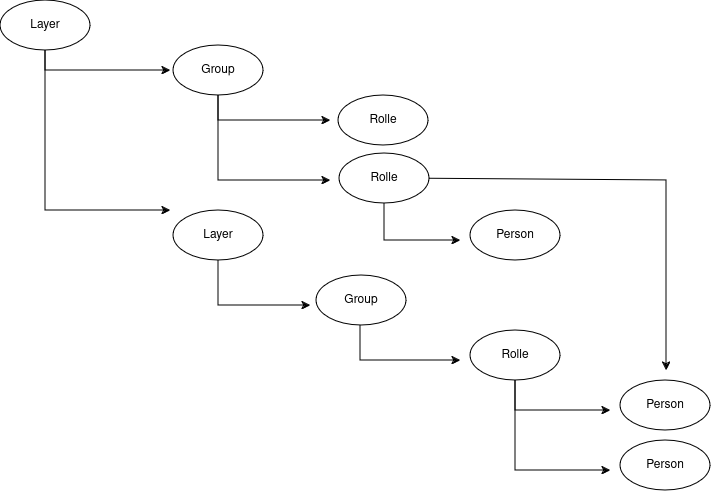
\includegraphics[width=1\textwidth,]{permissions_1.png}
  \caption{Gruppen und Ebenen, selbstgezeichnet mit Draw.io}
\end{figure}

Die Berechtigungen verwalten den Zugriff auf Layer und Gruppen. Ein Layer kann mehrere Gruppen haben,
eine Gruppe besitzt mehrere Rollen und eine Rolle kann wiederum mehrere Personen besitzen. Personen können
mehrere Rollen und somit eine Vielzahl von Berechtigungen besitzen.

\newpage

\subsection{Beispiel Zugriff Heinz}
\begin{figure}[h]
  \centering
  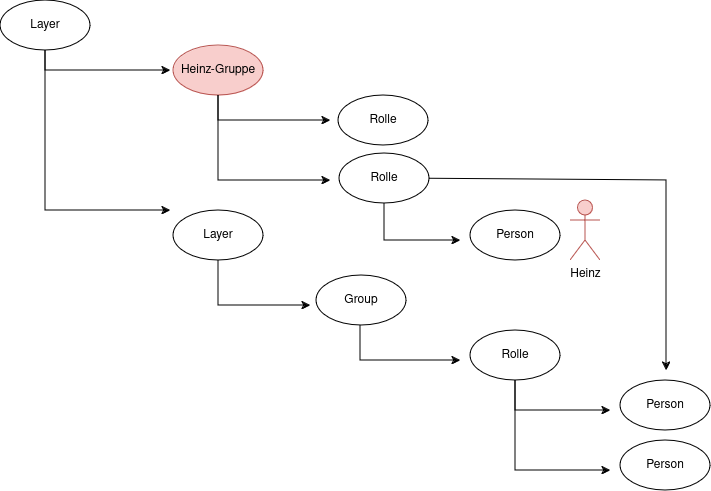
\includegraphics[width=1\textwidth,]{permissions_heinz.png}
  \caption{Beispiel Berechtigungen von Heinz, selbstgezeichnet mit Draw.io}
\end{figure}

Dieses Diagramm erklärt das Beispiel der Berechtigung "Group\_Full". Wir haben einen User namens Heinz
in unserem System. Heinz besitzt eine Rolle, welche mit der Heinz-Gruppe verknüpft ist. Die Rolle besitzt die Berechtigung "Group\_Full".

Dank dieser Verknüpfung besitzt Heinz Schreib- und Leserechte auf die Heinz-Gruppe.

\newpage

\subsection{Beispiel Zugriff Tim}
\begin{figure}[h]
  \centering
  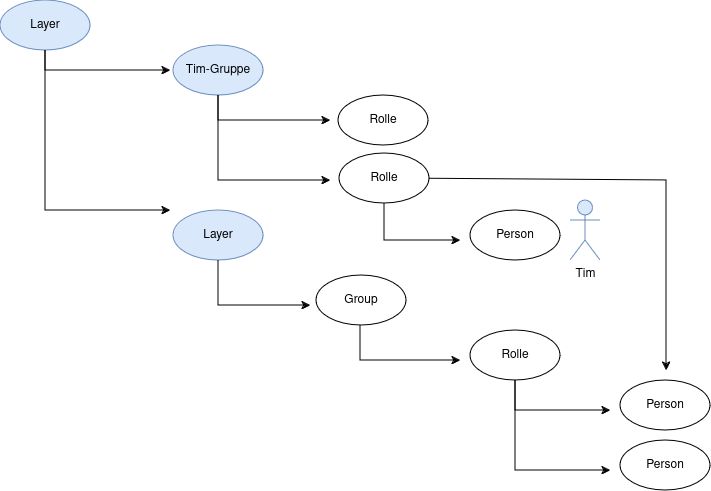
\includegraphics[width=1\textwidth,]{permissions_tim.png}
  \caption{Beispiel Berechtigungen von Tim, selbstgezeichnet mit Draw.io}
\end{figure}

Dieses Diagramm erklärt das Beipsiel der Berechtigung "Layer\_Full".  Wir haben einen User names Tim in unserem System.
Tim besitzt eine Rolle, welche mit der Tim-Gruppe verknüpft ist. Die Rolle besitzt die Berechtigung "Layer\_Full".

Durch diese Verknüpfung hat Tim Schreib- und Leserechte auf alle Gruppen, welche dem Layer seiner Gruppe unterliegen. 

\newpage

\subsection{Beispiel Zugriff Rudolf}
\begin{figure}[h]
  \centering
  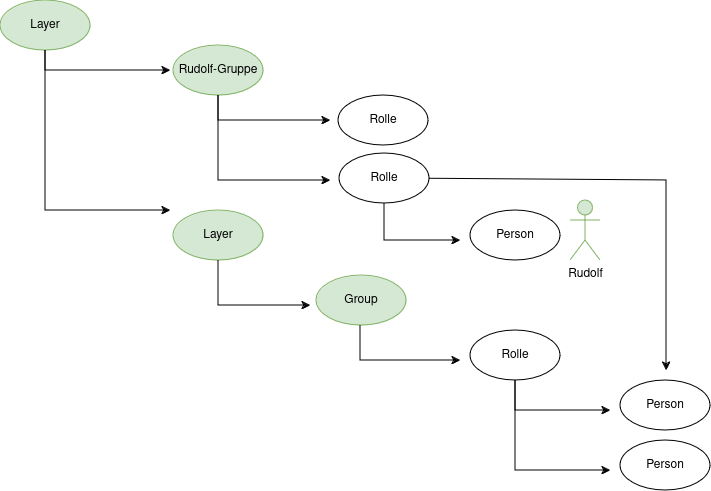
\includegraphics[width=1\textwidth,]{permissions_rudolf.png}
  \caption{Beispiel Berechtigungen von Tim, selbstgezeichnet mit Draw.io}
\end{figure}

Dieses Diagramm erklärt das Beispiel der Berechtigung "Layer\_Full\_And\_Below".  Wir haben einen Benutzer names Rudolf in unserem System.
Rudolf besitzt eine Rolle, welche mit der Rudolf-Gruppe verknüpft ist. Die Rolle besitzt die Berechtigung "Layer\_Full\_And\_Below".

Durch diese Verknüpfung hat Rudolf Schreib- und Leserechte auf alle Elemente, Layer und Gruppen, welche dem Layer der Rudolf-Gruppe unterliegen.

\subsection{Bedeutung für die Schnittstellen}
Durch die erklärten Berechtigungen, welche von den Rollen der Benutzern gegeben sind, werden die Rückgabewerte der Schnittstellen gefiltert.
Da im Rahmen dieser IPA eine Frontendanpassung gemacht wird, müssen bei der Berechtigungslogik keine Anpassungen gemacht werden. Die Berechtigungslogik wird
wie beschrieben verwendet.

\storeareas\riskvalues
\KOMAoptions{paper=a3, paper=landscape, DIV=current}
\areaset
  {\dimexpr\the\paperwidth-1cm\relax}
  {\dimexpr\the\paperheight-5.5cm\relax}
\recalctypearea

\subsection{Risikoanalyse}

\begin{table}[H]
  \begin{tabular}{ |C{0.01\textwidth}|C{0.1\textwidth}|C{0.1\textwidth}|C{0.02\textwidth}|C{0.02\textwidth}|C{0.04\textwidth}|C{0.1\textwidth}|C{0.2\textwidth}|C{0.02\textwidth}|C{0.02\textwidth}|C{0.04\textwidth}|C{0.1\textwidth}| }
      \hline
      \multirow{2}*{Nr} & \multirow{2}*{Risikobeschreibung} & \multirow{2}*{Auswirkung} & \multicolumn{4}{|l|}{Vor Massnahme}& \multirow{2}*{Massnahmen} & \multicolumn{4}{|l|}{Nach Massnahme} \\
      \cline{4-7} \cline{9-12}&&& W & S & Risiko & Handlungsweise &&  W & S & Risiko & Handlungsweise \\
      \hline 
      1 & \label{sec1} Daten ausserhalb der Berechtigung eines Benutzers werden angezeigt & Benutzer kann verbotene Informationen einsehen & W2 & S2 & \cellcolor{green}Niedrig & Risikominderung 
      & Daten werden vor dem Anzeigen im Filter anhand der Berechtigungen des Benutzers gefiltert & W1 & S1 & \cellcolor{green}Niedrig & Risikoakzeptanz \\
      \hline
      2 & \label{sec2} Benutzer kann einen Filter auf einer Ebene speichern, auf welcher er keinen Zugriff hat & Verwirrte Benutzer durch den neuen Filter & W2 & S2 & \cellcolor{green}Niedrig & Risikominderung 
      & Sicherstellen das der Benutzer nur Filter seiner Berechtigung entsprechend speichern kann. & W1 & S1 & \cellcolor{green}Niedrig & Risikoakzeptanz \\
      \hline
      3 & \label{sec3} SQL-Injection in ein Filter Eingabefeld (XSS) & Datenbank kann ausgelesen oder verändert werden & W4 & S4 & \cellcolor{red}Hoch & Risikominderung 
      & Alle Eingaben des Benutzers escapen & W2 & S1 & \cellcolor{green}Niedrig & Risikoakzeptanz \\
      \hline
      4 & \label{sec4} Bash-Injection in ein Filter Eingabefeld (XSS) & Schädliche Befehle werden serverseitig ausgeführt & W3 & S4 & \cellcolor{red}Hoch & Risikominderung 
      & Alle Eingaben des Benutzers escapen & W2 & S1 & \cellcolor{green}Niedrig & Risikoakzeptanz \\
      \hline
      5 & \label{sec5} Falsche Verwendung einer Library & Schwachstelle der Library kann von Angreifern ausgenutzt werden & W2 & S3 & \cellcolor{yellow}Mttel & Risikominderung 
      & Dokumentation der Libraries gut durchgehen, Libraries verwenden welche in der Rails Landschaft etabliert sind
       & W2 & S2 & \cellcolor{green} Niedrig & Risikoakzeptanz \\
      \hline
  \end{tabular}
  \caption{Risikoanalyse Sicherheitsrisiken}
\end{table}

\textbf{Schadensausmass:} \\
S1 = führt zu keinem Schaden am Projekt \\
S2 = führt zu geringem Schaden \\
S3 = hoher Schaden \\
S4 = führt zu schwerem Schaden am Projekt 
\newline
\newline
\textbf{Eintrittswahrscheinlichkeit:} \\
W1 = unvorstellbar \\
W2 = unwahrscheinlich \\
W3 = eher vorstellbar \\
W4 = vorstellbar \\
W5 = Eintreffen hoch \\

\restoregeometry
\riskvalues
\newpage

\section{Risikomatrix}
\begin{table}[H]
  \renewcommand{\arraystretch}{3.8}
  \begin{tabular}{*{6}{|L{0.16\textwidth}}}
      \hline
      W5 & \cellcolor{yellow}  & \cellcolor{red} &\cellcolor{red} & \cellcolor{red} \\
      \hline 
      W4 & \cellcolor{yellow} & \cellcolor{yellow} & \cellcolor{red} & \cellcolor{red} \tikz\draw[black,fill=white] circle [radius=0.2] node {3};  \\
      \hline
      W3 & \cellcolor{green} & \cellcolor{yellow} & \cellcolor{yellow} & \cellcolor{red}\tikz\draw[black,fill=white] circle [radius=0.2] node {4}; \\
      \hline 
      W2 & \cellcolor{green}\tikz\draw[black,fill=gray] circle [radius=0.2] node {3};\tikz\draw[black,fill=gray] circle [radius=0.2] node {5};\tikz\draw[black,fill=gray] circle [radius=0.2] node {4}; & \cellcolor{green} & \cellcolor{yellow}& \cellcolor{yellow}\tikz\draw[black,fill=white] circle [radius=0.2] node {5}; \cellcolor{yellow} \\
      \hline
      W1 & \cellcolor{green}\tikz\draw[black,fill=gray] circle [radius=0.2] node {1};\tikz\draw[black,fill=gray] circle [radius=0.2] node {2}; & \cellcolor{green} & \cellcolor{green} & \cellcolor{yellow} \\
      \hline
      & S1 & S2 & S3 & S4 \\
      \hline
  \end{tabular}
  \renewcommand{\arraystretch}{1}
  \caption{Risikomatrix Sicherheitsrisiken}
\end{table}

\textbf{Legende:}\\
\tikz\draw[black,fill=white] circle [radius=0.2] node {};  Risiko ohne Massnahme \\
\tikz\draw[black,fill=gray] circle [radius=0.2] node {};  Risiko nach Massnahme \\
\tikz\draw[black,fill=green] rectangle (0.3,0.3);  Geringes Risiko \\
\tikz\draw[black,fill=yellow] rectangle (0.3,0.3);  Mittleres Risiko \\
\tikz\draw[black,fill=red] rectangle (0.3,0.3);  Hohes Risiko \\

\section{Auswertung}
Die aufgeführten Risiken sowie die entsprechenden Massnahmen wurden mit den Stakeholdern besprochen
und von ihnen abgesegnet. Durch die Bestätigung der Stakeholder, werden die Massnahmen zur Risikominderung
in der Anforderungskatalog überführt.






\section{Anforderungen}
Alle Anforderungen an das Produkt werden im folgenden Abschnitt beschrieben. Die Priorisierung ist durch die Reihenfolge der 
Anforderungen gegeben. Somit erhält die erste Anforderung die höchste Priorität. Nicht funktionale und funktionale Anforderungen
werden als gleichwertig bewertet. Somit erhält die erste nicht funktionale Anforderung die gleiche Priorität wie die erste funktionale Anforderung.

\subsection{Nicht funktionale Anforderungen}

\begin{table}[h!]
   \begin{tabular}{|L{0.3\textwidth}|L{0.6\textwidth}|}
       \hline
       \rowcolor{puzzleblue} \multicolumn{2}{|l|}{\color{white}\textbf{Nicht funktionale Anforderung 1}} \\[4pt]
       \hline
       Beschreibung & Die Eingabefelder der Filter Benutzerschnittstelle unterbindet XSS Angriffe, gemäss \hyperref[sec3]{\color{blue}Sicherheitsrisiko 3} und \hyperref[sec4]{\color{blue}Sicherheitsrisiko 4}  \\
       \hline
       Messbarkeit & Benutzer können keine Bash, SQL oder sonstige Injections in das Eingabefeld einfügen.  \\
       \hline
     \end{tabular}
     \caption{Nicht funktionale Anforderung 1}
\end{table}

\begin{table}[h!]
   \begin{tabular}{|L{0.3\textwidth}|L{0.6\textwidth}|}
       \hline
       \rowcolor{puzzleblue} \multicolumn{2}{|l|}{\color{white}\textbf{Nicht funktionale Anforderung 2}} \\[4pt]
       \hline
       Beschreibung & Es werden im Rahmen der Implementation nur Libraries ohne nachweisbare Schwachstelle verwendet. Basiert auf \hyperref[sec5]{\color{blue}Sicherheitsrisiko 5}  \\
       \hline
       Messbarkeit & Es werden keine Schwachstellen bei den verwendeten Libraries gefunden.    \\
       \hline
     \end{tabular}
     \caption{Nicht funktionale Anforderung 2}
\end{table}

\begin{table}[h!]
   \begin{tabular}{|L{0.3\textwidth}|L{0.6\textwidth}|}
       \hline
       \rowcolor{puzzleblue} \multicolumn{2}{|l|}{\color{white}\textbf{Nicht funktionale Anforderung 3}} \\[4pt]
       \hline
       Beschreibung & Filterung soll ausschliesslich verfizierte Daten anzeigen, basiert auf \color{blue}\hyperref[sec1]{\color{blue} Sicherheitsrisiko 1}\color{black}  \\
       \hline
       Messbarkeit & Benutzer können keine Daten einsehen, auf welche sie keine Berechtigungen haben.  \\
       \hline
     \end{tabular}
     \caption{Nicht funktionale Anforderung 3}
\end{table}

\begin{table}[h!]
   \begin{tabular}{|L{0.3\textwidth}|L{0.6\textwidth}|}
       \hline
       \rowcolor{puzzleblue} \multicolumn{2}{|l|}{\color{white}\textbf{Nicht funktionale Anforderung 4}} \\[4pt]
       \hline
       Beschreibung & Speicherung von Filtern sind nur auf dem Benutzer zugänglichen Ebenen möglich. Basiert auf \color{blue}\hyperref[sec2]{\color{blue} Sicherheitsrisiko 2}\color{black}  \\
       \hline
       Messbarkeit & Filter welche vom Benutzer gespeichert werden, sind ausschliesslich auf seiner Ebene zugänglich.  \\
       \hline
     \end{tabular}
     \caption{Nicht funktionale Anforderung 4}
\end{table}

\begin{table}[h!]
   \begin{tabular}{|L{0.3\textwidth}|L{0.6\textwidth}|}
       \hline
       \rowcolor{puzzleblue} \multicolumn{2}{|l|}{\color{white}\textbf{Nicht funktionale Anforderung 5}} \\[4pt]
       \hline
       Beschreibung & Die gewählte Implementation der Überarbeit der Benutzerschnittstelle berücksichtigt, dass zukünftig
       weitere Filterkriterien dazu kommen können. \\
       \hline
       Messbarkeit & Es wird eine generische Methode zur Implementation gewählt, so dass zukünftige Filterkriterien nach dem 
       vorgegebenen Muster implementiert werden können.  \\
       \hline
     \end{tabular}
     \caption{Nicht funktionale Anforderung 5}
\end{table}

\begin{table}[h!]
   \begin{tabular}{|L{0.3\textwidth}|L{0.6\textwidth}|}
       \hline
       \rowcolor{puzzleblue} \multicolumn{2}{|l|}{\color{white}\textbf{Nicht funktionale Anforderung 6}} \\[4pt]
       \hline
       Beschreibung & Die Benutzerschnittstelle ist visuell ansprechend implementiert und folgt einem modularem Aufbau. Gemäss \hyperref[bed1]{Bedürfnis} aus Bedürfniserhebung \\
       \hline
       Messbarkeit & Es ist dem Benutzer möglich durch die hinterlegte Instruktion das Produkt zweckmässig zu verwenden.  \\
       \hline
     \end{tabular}
     \caption{Nicht funktionale Anforderung 6}
\end{table}

\newpage

\subsection{Funktionale Anforderungen}
\begin{table}[h!]
   \begin{tabular}{|L{0.3\textwidth}|L{0.6\textwidth}|}
       \hline
       \rowcolor{puzzleblue} \multicolumn{2}{|l|}{\color{white}\textbf{Funktionale Anforderung 1}} \\[4pt]
       \hline
       Beschreibung & Die Filterung bietet mit der neuen Implementation die gleiche Grundfunktionalität wie bisher. \\
       \hline
       Messbarkeit & Alle Funktionen welche in der Ist-Situation dokumentiert wurden, sind nach der Implementation immer noch vorhanden. \\
       \hline
       Testart & Manuell und Automatisiert \\
       \hline
     \end{tabular}
     \caption{Funktionale Anforderung 1}
\end{table}

\begin{table}[h!]
   \begin{tabular}{|L{0.3\textwidth}|L{0.6\textwidth}|}
       \hline
       \rowcolor{puzzleblue} \multicolumn{2}{|l|}{\color{white}\textbf{Funktionale Anforderung 2}} \\[4pt]
       \hline
       Beschreibung & Neue Filterkriterien können mit dem Hinzufüge-Button hinzugefügt werden. \\
       \hline
       Messbarkeit & Die beschriebene Funktion kann in der Benutzerschnittstelle ausgeführt werden. \\
       \hline
       Testart & Manuell und Automatisiert \\
       \hline
     \end{tabular}
     \caption{Funktionale Anforderung 2}
\end{table}

\begin{table}[h!]
   \begin{tabular}{|L{0.3\textwidth}|L{0.6\textwidth}|}
       \hline
       \rowcolor{puzzleblue} \multicolumn{2}{|l|}{\color{white}\textbf{Funktionale Anforderung 3}} \\[4pt]
       \hline
       Beschreibung & Die Bedingungen der Filterkriterien können über den Bearbeiten-Button editiert werden.  \\
       \hline
       Messbarkeit & Die beschriebene Funktion kann in der Benutzerschnittstelle ausgeführt werden. \\
       \hline
       Testart & Manuell und Automatisiert \\
       \hline
     \end{tabular}
     \caption{Funktionale Anforderung 3}
\end{table}

\begin{table}[h!]
   \begin{tabular}{|L{0.3\textwidth}|L{0.6\textwidth}|}
       \hline
       \rowcolor{puzzleblue} \multicolumn{2}{|l|}{\color{white}\textbf{Funktionale Anforderung 4}} \\[4pt]
       \hline
       Beschreibung & Neue Filterkriterien werden in Boxen anstatt von Dropdowns angezeigt. \\
       \hline
       Messbarkeit & Die beschriebene Funktion ist in der Benutzerschnittstelle ersichtlich. \\
       \hline
       Testart & Manuell und Automatisiert \\
       \hline
     \end{tabular}
     \caption{Funktionale Anforderung 4}
\end{table}

\begin{table}[h!]
   \begin{tabular}{|L{0.3\textwidth}|L{0.6\textwidth}|}
       \hline
       \rowcolor{puzzleblue} \multicolumn{2}{|l|}{\color{white}\textbf{Funktionale Anforderung 5}} \\[4pt]
       \hline
       Beschreibung & Das Filterkriterium ``Sprache'' wurde im Filterkriterium ``Felder'' untergebracht. Gemäss \hyperref[bed2]{\color{blue}Bedürfnis 2} aus Bedürfnisserhebung \\
       \hline
       Messbarkeit & Es besteht kein eigenes Filterkriterium ``Sprache'' mehr im Dropdown. \\
       \hline
       Testart & Manuell und Automatisiert \\
       \hline
     \end{tabular}
     \caption{Funktionale Anforderung 5}
\end{table}

\section{Abgrenzung}
Das Ziel dieser Arbeit ist es, eine komplette Überarbeitung der Benutzerschnittstelle von Personen- und Abonnementenfilter im Hitobito einzubauen.
Sämtliches Testing wird nur für die neue Benutzerschnittstelle gemacht, kaputte oder alte Tests werden deaktiviert und
kommentiert, sofern diese nichts mit der Implementation des Produktes zu tun haben. Diese Arbeit beschränkt sich auf die Überarbeitung der Benutzerschnittstelle des Personenfilters
und der Benutzerschnittstelle der globalen Bedingungen von Abonnementen. Andere Benutzerschnittstelle welche mit der Filterung verbunden sind,
werden erst nach der IPA überarbeitet.

Während dieser IPA wird die Funktionalität nur mit dem hitobito und hitobito\_generic Wagon garantiert. Alle anderen Wagons 
werden erst nach der IPA überprüft und ergänzt.

\section{Persönliche Vorgehensziele}

\chapter{Entwurf}
\section{Anwendungskonzept}
Im folgenden Abschnitt werden die Anwendungsfälle des Benutzers dokumentiert.

\subsection{Anwendungsdiagram}
\begin{figure}[h]
   \centering
   \fbox{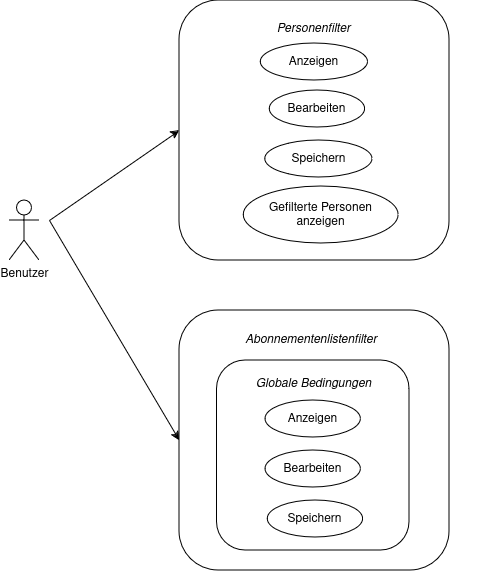
\includegraphics[width=0.6\textwidth,]{hitobito_use_case_diagram.png}}
   \caption{Anwendungsdiagram}
\end{figure}

\newpage

\subsection{Anwendungsfälle}
Aus dem Anwendungsdiagram werden die 4 Use-Cases entnommen und hier im Detail beschrieben. Vier Use-Cases, da die Anzeige,
die Bearbeitung und die Speicherung sowohl bei den Personenfiltern wie auch bei den Abonnementenfiltern über die gleiche Benutzerschnittstelle
läuft.

\begin{table}[h!]
   \begin{tabular}{|L{0.3\textwidth}|L{0.6\textwidth}|}
       \hline
       \rowcolor{puzzleblue} \multicolumn{2}{|l|}{\color{white}\textbf{Filter speichern}} \\[4pt]
       \hline
       Kurzbeschreibung & Der Benutzer kann die ausgewählten Filterkriterien speichern. \\
       \hline
       Vorbedingungen & 
       \begin{itemize}
         \item Der Benutzer besitzt die nötigen Rechte um eine Filter zu erstellen
         \item Mind. ein Filterkriterium wurde ausgewählt
       \end{itemize} \\
       \hline
       Ablauf & \begin{enumerate}
         \item Benutzer benennt den Filter, optional und nur bei der Filterung von Personen
         \item Benutzer klickt auf Speichern
       \end{enumerate}  \\
       \hline
       Resultat & Der Filter wurde in der Datenbank persistiert und ein Success-Alert wird ausgegeben. \\
       \hline
   \end{tabular}
   \caption{Anwendungsfall: Filter speichern}
\end{table}

\begin{table}[h!]
   \begin{tabular}{|L{0.3\textwidth}|L{0.6\textwidth}|}
      \hline
      \rowcolor{puzzleblue} \multicolumn{2}{|l|}{\color{white}\textbf{Filterkriterien anzeigen}} \\[4pt]
      \hline
      Kurzbeschreibung & Der Benutzer kann die Filterkriterien der gespeicherten Filter einsehen. \\
      \hline
      Vorbedingungen & 
      \begin{itemize}
         \item Der Benutzer hat einen Filter gespeichert
      \end{itemize}  \\
      \hline
      Ablauf & \begin{enumerate}
      \item Navigiert zum Filter
      \end{enumerate}  \\
      \hline
      Resultat & Die Filterkriterien werden dem Benutzer angezeigt. \\
      \hline
   \end{tabular}
   \caption{Anwendungsfall: Filterkriterien anzeigen}
\end{table}

\newpage

\begin{table}[h!]
   \begin{tabular}{|L{0.3\textwidth}|L{0.6\textwidth}|}
      \hline
      \rowcolor{puzzleblue} \multicolumn{2}{|l|}{\color{white}\textbf{Filterkriterien bearbeiten}} \\[4pt]
      \hline
      Kurzbeschreibung & Der Benutzer kann die Filterkriterien die Filterkriterien bearbeiten. \\
      \hline
      Vorbedingungen & 
      \begin{itemize}
         \item Der Benutzer hat einen Filter gespeichert
      \end{itemize}  \\
      \hline
      Ablauf & \begin{enumerate}
      \item Der Benutzer klickt auf den Bearbeiten-Button
      \end{enumerate}  \\
      \hline
      Resultat & Die Filterkriterien werden dem Benutzer angezeigt. \\
      \hline
   \end{tabular}
   \caption{Anwendungsfall: Filterkriterien bearbeiten}
\end{table}

\begin{table}[h!]
   \begin{tabular}{|L{0.3\textwidth}|L{0.6\textwidth}|}
      \hline
      \rowcolor{puzzleblue} \multicolumn{2}{|l|}{\color{white}\textbf{Personen filtern}} \\[4pt]
      \hline
      Kurzbeschreibung & Der Benutzer kann die definierten Personenfilter auf eine Liste von Personen 
      anwenden. \\
      \hline
      Vorbedingungen & \begin{itemize}
         \item Benutzer besitzt Rechte um auf eine Personenliste zuzugreifen
         \item Benutzer hat einen Personenfilter für diese Liste gespeichert
         \end{itemize}  \\
      \hline
      Ablauf & \begin{enumerate}
      \item Benutzer Navigiert zum Personenfilter
      \item Benutzer klickt auf den Filternamen
      \end{enumerate}  \\
      \hline
      Resultat & Die Personen in der Personenliste werden gefiltert und dem Benutzer angezeigt. \\
      \hline
   \end{tabular}
   \caption{Anwendungsfall: Personen filtern}
\end{table}

\newpage

\section{Systemkonzept}
Bei dieser Arbeit wird mit einem bestehenden System gearbeitet, dieses muss entsprechend angepasst werden. 
Um die nötigen Anpassungen besser sichtbar zu machen, werden im folgenden Abschnitt die Betroffenen Services identifiziert.
Anschliessen werden mögliche Lösungsvarianten konzeptioniert. Aus den Lösungsvarianten wird per Variantenentscheid eine Lösungsvariante ausgearbeitet.

\begin{figure}[h]
   \centering
   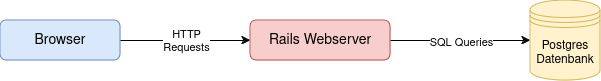
\includegraphics[width=1\textwidth,]{hitobito_systemarchitektur.drawio.png}
   \caption{Services}
\end{figure}

\subsection{Betroffene Services}
Hitobito wird in zwei Services unterteilt, der Rails Applikation und der Postgres Datenbank.

\textbf{Rails Applikation / Webserver}

Die Rails Applikation verwaltet die Geschäftslogik von Hitobito. Die Erweiterugnen dieser Arbeit
werden alle in diesem Service vorgenommen. Je nach Kunde werden hier Codeteile aus den anderen Wagons verwendet.
In dieser Arbeit wird ausschliesslich der Core und der Generic Wagon angepasst.

\textbf{Postgres Datenbank}

Die Datenbank von Hitobito läuft auf PostgreSQL. Sämtliche Abfragen auf die PostgreSQL Datenbank werden via SQL-Queries
gemacht. Als ORM (Object Relational Mapping) wird Active Record verwendet.

\newpage

\subsection{Lösungsvarianten}

\textbf{Lösungsvariante 1}

Die Idee des nachfolgenden Konzeptes ist die Aufteilung des Mockups in Elemente, welche später durch 
Turbo angesteuert werden können. Hierbei sollen nur Turbo-Streams verwendet werden. Diese ermöglichen uns Element nur mit der ID 
eines Divs, zu diesem Div hinzuzufügen.  

\begin{figure}[h]
   \centering
   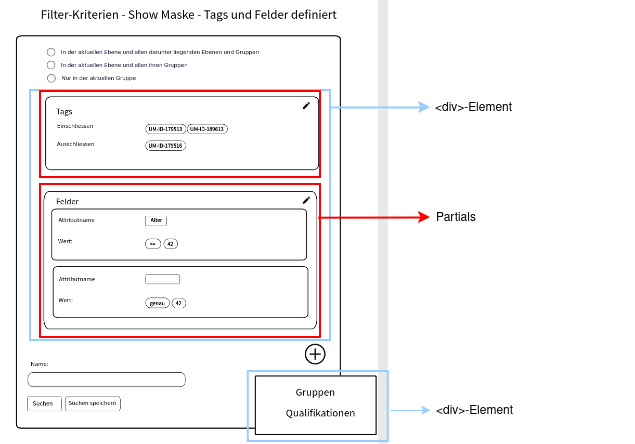
\includegraphics[width=1\textwidth,]{variant_one_turbo.png}
   \caption{Lösungsvariante 1: Turbo-Konzept}
\end{figure}

So werden keine Turboframes benötigt und es müssen lediglich nur noch die Endpoints angepasst werden.

\newpage

Das daraus resultierende Klassendiagramm sieht so aus:

\begin{figure}[h]
   \centering
   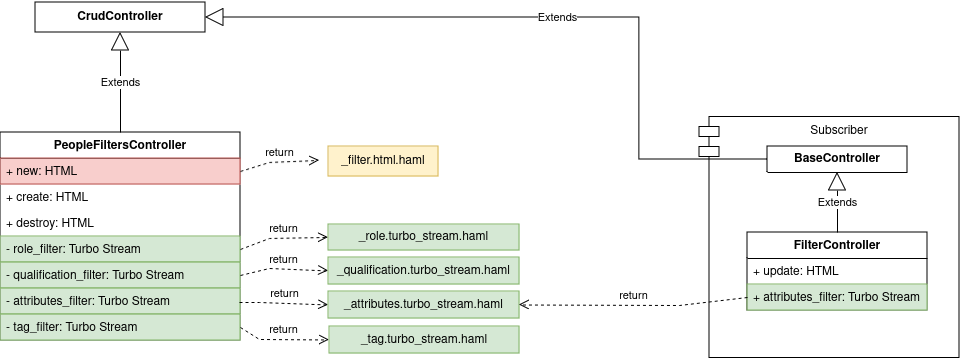
\includegraphics[width=1\textwidth,]{variant_one_class_structure.png}
   \caption{Lösungsvariante 1: Klassendiagramm}
\end{figure}

Rot markierte Felder stehen dabei für Funktionen, welche entfernt werden. Grün steht für Funktionen, welche hinzugefüt werden.
Gelb steht für Funktionen oder Dateien, welche bearbeitet werden müssen.

Im \texttt{PeopleFilterController} wie im \texttt{FilterController} werden zusätzliche Endpoints angelegt
welche die jeweilgen Partials als Turbostream zurückgeben. Mit den Turbo Streams werden die Partials einem texttt{div} angehängt oder
von diesem entfernt. Da die Filterkriterien mittels der Turbostream angezeigt werden, wird der Endpoint ``new'' im \texttt{PeopleFilterController}
nicht mehr benötig. Die View \texttt{\_filter.html.haml} muss so geändert werden, dass sie alle Boxen welche durch die Filterungskriterien
auf der Benutzerschnittstelle darstellen, in ein \texttt{Div} verpackt. Dieses \texttt{Div} kann später in den 
Turbostreams referenziert werden.

\newpage

\textbf{Lösungsvariante 2}

In der zweiten Lösungsvariante wird mit Turboframes statt der Turbostreams gearbeitet. Für jedes Partial besteht zu Beginn ein
Turboframe. Wird im Dropdown auf eines der Filterkriterien geklickt, der Inhalt des Turboframes mit dem Formular für das jeweilige 
Filterkriterium befüllt.

\begin{figure}[h]
   \centering
   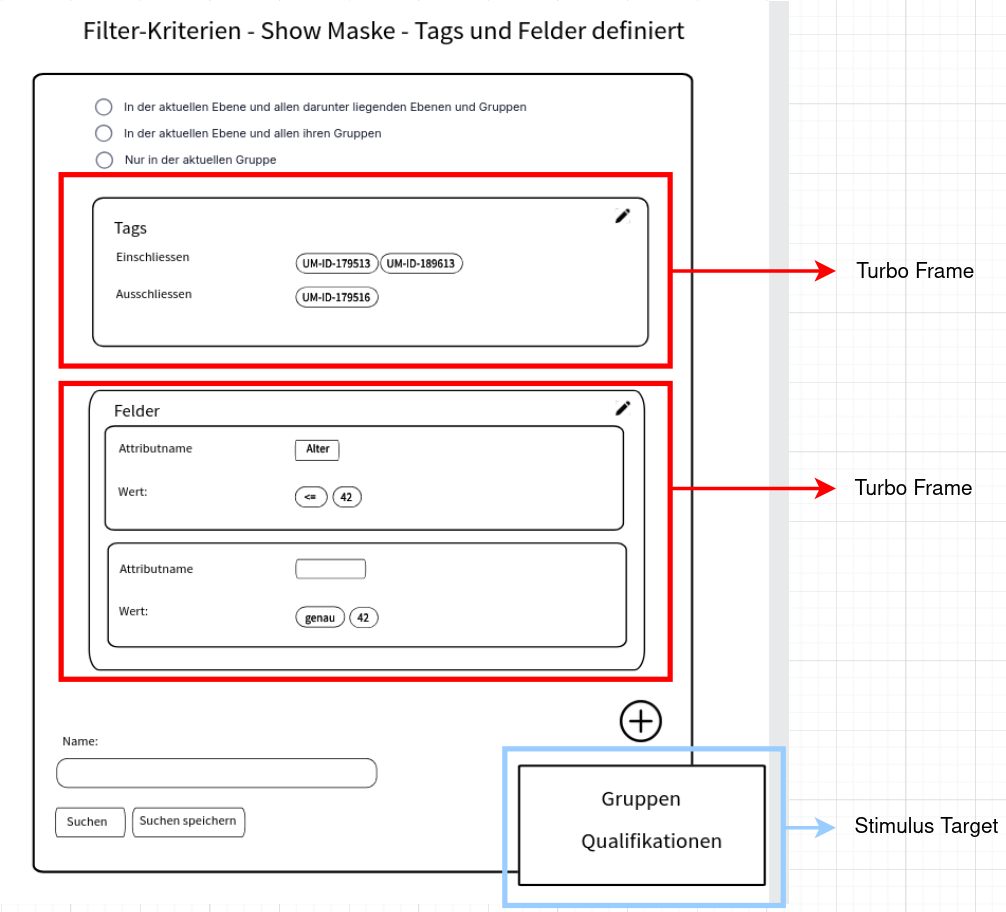
\includegraphics[width=1\textwidth,]{variant_two_turbo_concept.png}
   \caption{Lösungsvariante 2: Turbo-Konzept}
\end{figure}

Die Option im Dropdown wird durch einen Stimulus Controller entfernt. So muss kein zusätzliches 
Turboframe für das Dropdown angelegt werden. 

\newpage

Eine Umsetzung dieses Turbo-Konzeptes führt zu folgendem Klassendiagramm.

\begin{figure}[h]
   \centering
   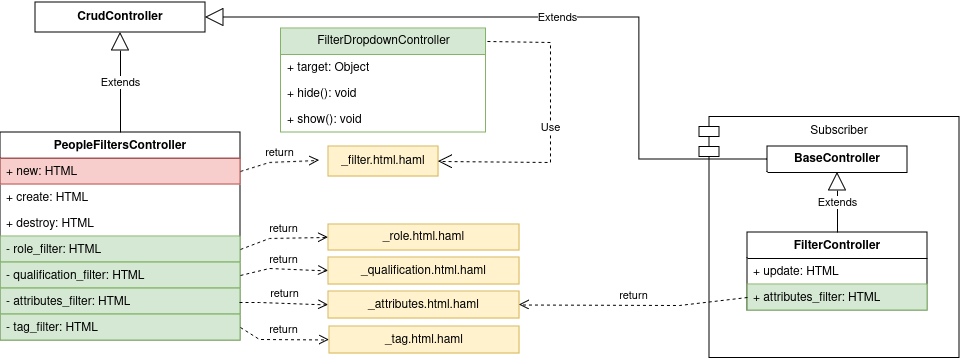
\includegraphics[width=1\textwidth,]{variant_two_class_structure.png}
   \caption{Lösungsvariante 2: Klassendiagramm}
\end{figure}

Massgebend ist der Unterschied, dass hier keine Turbostreams benötigt werden. Es wird nach wie vor für jedes Filterkriterium ein
ein Endpoint erstellt. Diese liefern allerdings die bereits bestehenden Partials zurück. An den Partials selbst muss ein Turboframe eingebaut werden.
So wird jedes Form eines Filterkriteriums von einem Turboframe umschlossen. Als zusätzliche Klasse entsteht in dieser Variante der \texttt{FilterDropdownController}.
Die Aufgabe dieses Controllers ist es, die Filterkriterien bei der Auswahl aus dem Dropdown zu entfernen. Wurden alle Filterkriterien ausgewählt blendet der Controller das
Dropdown komplett aus. 

\newpage

\subsection{Variantenentscheid}
Um eine geeignete Entscheidung für eine der beschriebenen Lösungsvarianten zu treffen, wird eine Bewertungsmatrix verwendet. Die Bewertungsmatrix
bewertet die Lösungsvarianten nach definierten Kriterien. Die Kriterien können mit Punkten von 1 bis 10 bewertet werden, wobei 1 Punkt für das Nicht-Erfüllen
eines Kriteriums und 10 für das Erfüllen des Kriteriums steht. 

Folgende Kriterien wurden definiert:

\begin{table}[h!]
   \begin{tabular}{|L{0.2\textwidth}|L{0.3\textwidth}|L{0.2\textwidth}|L{0.2\textwidth}|}
      \hline
      \rowcolor{puzzleblue}{\color{white} \textbf{Kriterium}} & \color{white}\textbf{Beschreibung} & \color{white}\textbf{1 Punkt} & \color{white}\textbf{10 Punkte} \\[2pt]
      \hline
      Zeitaufwand & Wie viel Zeit wird für die Implementation benötigt? 
      & Grosser Zeitaufwand, IPA ist mit diesem Konzept nicht umsetzbar. & Kleiner Zeitaufwand, IPA ist problemlos umsetzbar. \\
      \hline
      Einführung & Ist das Konzept einfach in die produktive Umgebung einzuführen? Müssen Migrationen vorgenommen werden?
       & Einführung in produktive Umgebung ist unmöglich. & Einführung in produktive Umgebung ist problemlos möglich.\\
      \hline
      Anforderungen & Kann mit dieser Variante jede Anforderung erfüllt werden?
      & Mehrere Anforderung können nicht erfüllt werden. & Alle Anforderunge können erfüllt werden. \\
      \hline
      Performanz & Ist das Konzept performant? Spart das Konzept Zeit / Requests? 
      & Konzept ist nicht performant, Filterungen sind durch Implementation deutlich langsamer.
      & Es wird viel Zeit durch die Implementation des Konzepts gespart.\\
      \hline
   \end{tabular}
   \caption{Variantenentscheid Kriterien}
\end{table}

\newpage

\textbf{Bewertungen}

Im folgenden Abschnitt werden den definierten Kriterien Gewichtungen hinzugefüht, da nicht jedes Kriterium gleich wichtig für
diese IPA ist.

\textbf{Gewichtungen in \%}

\begin{itemize}
   \item \textbf{Zeitaufwand 40\%:} Um eine funktionelle Lösung am Ende der IPA aufweisen zu können, wird dem Zeitaufwand eine hohe Gewichtung zugerodnet.
   \item \textbf{Einführung 20\%:} Es ist wichtig eine Lösung zu implementieren welche schnell ihren Weg in die produktive Umgebung finden, da die Einführung von der IPA ausgenommen ist, wird diesem Kriterium eine geringere Gewichtung zugeordnet.
   \item \textbf{Anforderungen 30\%:} Damit die definierten Anforderungen an das Produkt erfüllt werden können und die Erfüllung zur Endnote der IPA beiträgt, wird diesem Kriterium eine hohe Gewichtung zugeordnet. 
   \item \textbf{Performanz 10\%: } Ist eine Applikation zu langsam und benötigt mehrere Minute bis sie Resultate geladen hat, kann das den Benutzer schnell vor den Kopf stossen und dafür führen das dieser die Applikation in Zukunft nicht mehr verwendet.
\end{itemize}

\textbf{Lösungsvariante 1}

\begin{table}[h!]
   \begin{tabular}{|L{0.2\textwidth}|L{0.2\textwidth}|L{0.6\textwidth}|}
      \hline
      \rowcolor{puzzleblue}{\color{white} \textbf{Kriterium}} & \color{white}\textbf{Bewertung} & \color{white}\textbf{Beschreibung}\\[2pt]
      \hline
      Zeitaufwand & 5 & Mittlerer Zeitaufwand. Durch die vielen Neuimplementationen der Turbostreams geht viel Zeit verloren. \\
      \hline
      Einführung & 8 & Einführung möglich, es werden keine grossen Schwierigkeiten auftreten. \\
      \hline 
      Anforderungen & 10 & Alle Anforderung können potentiell durch diese Lösungsvariante erfüllt werden. \\
      \hline
      Performance & 8 & Performanz wird optimiert. \\
      \hline
   \end{tabular}
   \caption{Bewertung Lösungsvariante 1}
\end{table}

\newpage

\textbf{Lösungsvariante 2}

\begin{table}[h!]
   \begin{tabular}{|L{0.2\textwidth}|L{0.2\textwidth}|L{0.6\textwidth}|}
      \hline
      \rowcolor{puzzleblue}{\color{white} \textbf{Kriterium}} & \color{white}\textbf{Bewertung} & \color{white}\textbf{Beschreibung}\\[2pt]
      \hline
      Zeitaufwand & 6 & Durch weniger Neuimplementationen kann viel Zeit gespart werden. \\
      \hline
      Einführung & 6 & Einführung möglich, könnte aufgrund des Einsetzens von Turboframes in den bereits bestehenden Partials Probleme ergeben. \\
      \hline 
      Anforderungen & 10 & Alle Anforderung können potentiell durch diese Lösungsvariante erfüllt werden. \\
      \hline
      Performance & 7 & Performanz wird optimiert, jedoch weniger als es mit den Turbostreams möglich ist. \\
      \hline
   \end{tabular}
   \caption{Bewertung Lösungsvariante 2}
\end{table}

\newpage
\storeareas\bruteforceanalysis
\KOMAoptions{paper=a4, paper=landscape, DIV=current}
\areaset
  {\dimexpr\the\paperwidth-3cm\relax}
  {\dimexpr\the\paperheight-7.5cm\relax}
\recalctypearea

\begin{table}[H]
  \begin{tabular}{|L{0.12\textwidth}|L{0.12\textwidth}|L{0.15\textwidth}|L{0.15\textwidth}|L{0.15\textwidth}|L{0.15\textwidth}|}
        \hline
        \rowcolor{puzzleblue} \multicolumn{2}{|l|}{} & \multicolumn{2}{|l|}{\color{white}Lösungsvariante 1: Turbostreams} & \multicolumn{2}{|l|}{\color{white}Lösungsvariante 2: Turboframes} \\ [10pt]
        \hline
        \multirow{2}{*}{Kriterium} & \multirow{2}{*}{Gewichtung} & \multirow{2}{*}{Ungewichtet} & \multirow{2}{*}{Gewichtet} & \multirow{2}{*}{Ungewichtet} & \multirow{2}{*}{Gewichtet} \\ [10pt]
        \hline
        \multirow{2}{*}{Zeitaufwand} & \multirow{2}{*}{40\%} & \multirow{2}{*}{5} & \multirow{2}{*}{2} & \multirow{2}{*}{6} & \multirow{2}{*}{2.4} \\ [10pt]
        \hline
        \multirow{2}{*}{Einführung} & \multirow{2}{*}{20\%} & \multirow{2}{*}{8} & \multirow{2}{*}{1.6} & \multirow{2}{*}{6} & \multirow{2}{*}{1.2} \\ [10pt]
        \hline
        \multirow{2}{*}{Anforderungen} & \multirow{2}{*}{30\%} & \multirow{2}{*}{10} & \multirow{2}{*}{3} & \multirow{2}{*}{10} & \multirow{2}{*}{3} \\ [10pt]
        \hline
        \multirow{2}{*}{Performanz} & \multirow{2}{*}{10\%} & \multirow{2}{*}{8} & \multirow{2}{*}{0.8} & \multirow{2}{*}{7} & \multirow{2}{*}{0.7} \\ [10pt]
        \hline
        \multirow{2}{*}{Total} & \multirow{2}{*}{100\%} & \multirow{2}{*}{31} & \multirow{2}{*}{7.4} & \multirow{2}{*}{29} & \multirow{2}{*}{7.3} \\ [10pt]
        \hline
    \end{tabular}
    \caption{Nutzwertanalyse}
\end{table}

\textbf{Fazit}
Durch die bessere Möglichkeit zur Einführung und der erhöhten Performanz hat die Lösungsvariante 1 die Lösungsvariante 2 in der Endbewertung knapp übertroffen.
Für die Implementation wird fortlaufend die Lösungsvariante 2 verwendet.

\restoregeometry
\bruteforceanalysis
\newpage

\section{Sicherheitskonzept}
Um die Sicherheit im Umbau der Filter sicherzustellen wird ein Sicherheitskonzept
benötigt. Das Ziel dieses Konzeptes ist es mögliche Angriffe aufzuführen
und die Blockade dieser Angriffe zu dokumentieren. 

\subsection{SQL-Injection}
Die Einzigen Benutzereingabe welche in dieser IPA auftritt, ist die Texteingabe im Filterkriterium ``Felder''. 
Da die Eingabe des Benutzers nicht direkt in die Postgres Datenbank gespeichert wird,
ist diese Eingabe nicht für eine SQL-Injection gefährdet. Selbst wenn die SQL-Abfrage direkt gemacht würde,
verhindert das ORM ActiveRecord mit seinen Standardmethoden, dass schädliche Eingaben abgespeichert werden.
Dies geschieht unter anderem durch das Escapen der Strings.

\subsection{Cross-Site Scripting}
Da in dieser Erweiterung Benutzereingaben an das Rails-Backend gesendet werden muss der Cross-Site Scripting Angriff ebenfalls
berücksichtig werden. Rails selbst bietet dafür einen eingebauten Abwehrmechanismus. Eine solcher XSS-Angriff kann folgendermassen aussehen:

\begin{lstlisting}[language=HTML]
   <h2>Welcome <script>alert("This is a XSS attack!")</script></h2>
\end{lstlisting}

Standardmässig escaped Rails diese Eingaben und ändert die Spezialbuchstaben. So wird aus der Eingabe oben:

\begin{lstlisting}[language=HTML]
   <h2>Welcome &lt;script&gt;alert\
   (&quot;This is a XSS attack!&quot;)&lt;/script&gt;</h2>
\end{lstlisting}

\subsection{URL Interpretation}
Bei der URL-Interpretation fabriziert der Angreifer eine URL um damit auf die persönlichen
Daten eines Benutzers zuzugreifen. Dabei kann der Angreifer versuchen die URL zu erraten. 
Dieser Angriff wird in Hitobito mit dem Gem \texttt{can-can-can} verhindert. Mit diesem Gem wird sichergestellt,
das der Absender der Anfrage die nötigen Berechtigungen für das Einsehen der Informationen hat. Die Prüfung der Berechtigungen sieht wie folgt
aus: 

\begin{lstlisting}[language=Ruby]
   class Ability include CanCan::Ability
      def define_root_abilities
         can :manage, :all
         # root cannot change her email, because this is what makes her root.
         cannot :update_email, Person do |p|
            p.root?
      end
   end
\end{lstlisting}
   
\subsection{Kommunikation HTTP/S}
Die Umgebungen auf der Integration und Produktion kommunizieren via HTTPS. Somit ist
die verschlüsselte Kommunikation beim Transfer von produktiven Daten gesichert.

\section{Fehlerbehandlungskonzept}
Bei der Entwicklung und während der Laufzeit können stets Fehler oder nicht vorgesehene Probleme entstehen.
Im folgenden Abschnitt wird dokumentiert, wie mit diesen Fällen umgegangen wird.

\subsection{Nutzereingabe}
Bei der Nutzereingabe des Users werden keine möglichen Exceptions erwartet. Der Benutzer kann im Filter, in der Suche nach einem
bestimmten Text alles eingeben, ohne Einschränkungen. Mögliche Angriffe werden gemäs den definierten \hyperref[sec1]{\color{blue}Sicherheitsmassnahmen} behandelt. 

\subsection{Laufzeitfehler}
Tritt in der Applikation ein Laufzeit Fehler auf, wird dies sowohl in den Log,s wie in der Sentry
Umgebung von Hitobito aufgezeigt. Im Sentry werden zusätzlich die aufgetretenen Execptions gesammelt, um 
den Entwicklern eine Übersicht über allfällige Bugs zu geben. Gesammelte Exceptions können einem Entwickler
zugewiesen oder wenn sie gefixed wurden, vom Sentry entfernt werden. Für diese IPA ist keine Modifizierung an der 
Sentry Umgebung nötig.

\subsection{Exception Handling}
In Ruby können Exception mit \texttt{rescue} abgefangen werden. Das folgende Beispiel macht das Exceptionhandling anhand eines 403 Fehlers bei
Zugriff auf einen nicht erlaubten Endpoint sichtbar.

\begin{lstlisting}[language=Ruby]
   rescue_from CanCan::AccessDenied do |exception|
    respond_to do |format|
      format.json do
        render json: {status: 403, error: I18n.t("devise.failure.not_permitted_to_view_page")},
          status: 403
      end
      format.all do
        raise exception unless Rails.env.production?
        redirect_to root_path, alert: I18n.t("devise.failure.not_permitted_to_view_page")
      end
    end
  end
\end{lstlisting}

Sobald die \texttt{AccessDenied} Exception geworfen wird, wird diese vom \texttt{ApplicationController}
in Hitobito abgefangen. Im Rahmen dieser IPA kann diese Exception vorkommen, wenn ein Benutzer versucht, die Filterung
von Personen einzusehen auf welche er keine Berechtigungen hat. Im Rahmen dieser IPA wird auf das bestehende Exceptionhandling zurückgegriffen.
Es wird kein zusätzliches Exceptionhandling benötigt.

\newpage

\section{Testsetup}
Um im Hitobito Tests ausführen zu können wird folgendes Setup benötigt:

\begin{itemize}
   \item Bash-Konsole
   \item Docker oder Docker Desktop bei Windows als OS. 
   \item Geklontes Github Repository von \url{https://github.com/hitobito/development.git}.
   \item Core Wagon wurde in das Verzeichnis \texttt{/app} unter dem geklonten Development Repository eingefügt. Core Wagon kann unter \url{https://github.com/hitobito/hitobito.git} geklont werden.
   \item Generic Wagon wurde in das Verzeichnis \texttt{/app} unter dem geklonten Development Repository eingefügt. Generic Wagon kann unter \url{https://github.com/hitobito/hitobito_generic.git} geklont werden.
\end{itemize}

Besteht das beschriebene Setup muss zur Ausführung der Tests in das Development Repository navigiert werden. Dort müssen folgende Befehle der Reihe nach wie hier 
beschrieben ausgeführt werden:

\label{testsetup}
\begin{itemize}
   \item \texttt{bin/dev-env.sh} - Startet Hitobito Konsole
   \item \texttt{hit test prep} - Bereitet Tests vor, kompiled Assets
   \item \texttt{hit test} - Führt Migrationen durch, bereitet Testumgebung vor
   \item \texttt{rspec <path\_to\_tests>} Variable in Klammern muss durch den Pfad zu den Tests ersetzt werden. Wird ein Ordner unter dem Pfad angegeben, werden alle Tests unter diesem Ordner ausgeführt.
\end{itemize}

\newpage

\section{Testkonzept}
\subsection{Testinfrastruktur}
Es gibt zwei Arten von Tests, welche in dieser Arbeit relevant sind:

\begin{itemize}
   \item \textbf{Feature Tests:} Testet eine Funktion über die Benutzerschnittstelle
   \item \textbf{Manuelles Testen:} Testet das gesamte Feature
\end{itemize}

Hitobito verwendet für das Ausführen lokaler Tests RSpec 3.13.0. Für die manuellen Tests wird Firefox 80.0 (64-bit) verwendet. Als Gerät wird ein Laptop mit Pop!\_OS 22.04 LTS verwendet.

Die bestehenden Tests welche die Funktionalität der gesamten Applikation sicherstellen werden für das Testing vernachlässigt. Es werden keine Anpassungen
an diesen Tests vorgenommen. Die bestehenden Tests werden aus zeitlichen Rahmen bei Fehlschlagen auskommentiert und ignoriert. Im Rahmen dieser Arbeit sind
auschliesslich die selbst verfassten Tests relevant.

\subsection{Fehlerklassen}
\begin{table}[h!]
   \begin{tabular}{|L{0.2\textwidth}|L{0.4\textwidth}|L{0.4\textwidth}|}
       \hline
       \rowcolor{puzzleblue} \color{white}\textbf{Bezeichnung} & \color{white}\textbf{Fehlerklasse} & \color{white}\textbf{Beschreibung} \\[12pt]
       \hline
       FK0 & Fehlerfrei & Keine Fehler \\
       \hline
       FK1 & Nicht erfolgsgefährdend & Kleine Fehler, beeinträchtigen Funktion nur bedingt. \\
       \hline
       FK2 & Erfolgsgefährdend & Fehler welche die Funktion beeinträchtigen. \\
       \hline
     \end{tabular}
     \caption{Fehlerklassen}
\end{table}

\subsection{Manuelle Tests}
Die manuellen Tests werden lokal, mit den Testdaten von Hitobito durchgeführt. Die Testdaten können in der Hitobito-Konsole
mit \texttt{hit rails wagon seed} eingespielt werden. Bei Fragen zur Aktvierung der Hitobito Konsole, den \hyperref[testsetup]{\color{blue}Beschrieb zum Testsetup} einsehen.

\newpage

Mit dem generic Wagon bietet sich ein Benutzer-Account für das Login an:

\begin{table}[h!]
   \begin{tabular}{|L{0.2\textwidth}|L{0.3\textwidth}|L{0.2\textwidth}|L{0.4\textwidth}|}
       \hline
       \rowcolor{puzzleblue} \color{white}\textbf{Bezeichnung} & \color{white}\textbf{Username} & \color{white}\textbf{Passwort} & \color{white}\textbf{Berechtigungen}\\[12pt]
       \hline
        Admin & admin@hitobito.ch & demo & Administrator mit vollem Zugriff \\
       \hline
     \end{tabular}
     \caption{Accounts für manuelle Tests}
\end{table}

Bei den manuellen Tests muss stets einer der oben beschriebenen Accounts verwendet werden.
In den Testszenarien wird der Account mit ``Als \{Account\} anmelden'' beschrieben. \{ Account \} steht hierbei als
Platzhalter für den Account des jeweiligen Benutzer. 
Das Login basiert auf folgendem Ablauf:

\begin{itemize}
   \item Navigation auf \texttt{localhost:3000/users/sign\_in}
   \item Anmeldedaten des Accounts eingeben
   \item Auf Anmelde-Button klicken
\end{itemize}

\newpage

\begin{table}[h!]
   \rowcolors{2}{puzzleblue!30}{white}
   \begin{tabular}{|L{0.4\textwidth}|L{0.6\textwidth}|}
       \hline
       \rowcolor{puzzleblue} \multicolumn{2}{|l|}{\color{white}\textbf{Testfall Nr. 1}} \\[12pt]
       \hline
        Testname & Personenfilter anzeigen \\
       \hline
       Testmethode & Manuell \\
       \hline
        Anforderung & \begin{itemize}
         \item Nicht funktionale Anforderung 6
         \item Funktionale Anforderung 1
         \item Funktionale Anforderung 4
         \end{itemize}  \\
       \hline
       Voraussetzungen & Ein eigener Personenfilter wurde erfasst und gespeichert \\
       \hline
       Testszenario & 
       \begin{itemize}
         \item Als Admin anmelden
         \item Mittels Reiter ``Personen'' auf Personenliste navigieren
         \item Maus Im Filter Dropdown über dem Namen des Filters positionieren
         \item Erscheinende Option ``Bearbeiten'' auswählen
       \end{itemize} \\
       \hline
       Erwartetes Resultat & 
       \begin{itemize}
         \item Alle Filterkriterien un deren Bedingungen werden angezeigt
      \end{itemize} \\
      \hline
     \end{tabular}
     \caption{Testfall 1}
\end{table}

\newpage

\begin{table}[h!]
   \rowcolors{2}{puzzleblue!30}{white}
   \begin{tabular}{|L{0.4\textwidth}|L{0.6\textwidth}|}
       \hline
       \rowcolor{puzzleblue} \multicolumn{2}{|l|}{\color{white}\textbf{Testfall Nr. 2}} \\[12pt]
       \hline
        Testname & Filterkriterium ``Tags'' bearbeiten \\
       \hline
       Testmethode & Manuell \\
       \hline
        Anforderung & 
        \begin{itemize}
         \item Nicht funktionale Anforderung 6
         \item Funktionale Anforderung 1
         \item Funktionale Anforderung 3
         \end{itemize}  \\
       \hline
       Voraussetzungen & Ein eigener Personenfilter wurde erfasst und gespeichert \\
       \hline
       Testszenario & 
       \begin{itemize}
         \item Als Admin anmelden
         \item Mittels Reiter ``Personen'' auf Personenliste navigieren
         \item Maus Im Filter Dropdown über dem Namen des Filters positionieren
         \item Erscheinende Option ``Bearbeiten'' auswählen
         \item Auf Box des Filterkriteriums ``Tags'' navigieren
         \item Bearbeiten-Button in der oberen rechten Ecke klicken
         \item ``Puzzle ITC'' als ``Tag'' bei dem Eingabefeld ``Einschliessen'' hinzufügen
         \item Speichern-Button innerhalb der Box des Filterkriteriums klicken
       \end{itemize} \\
       \hline
       Erwartetes Resultat & 
       \begin{itemize}
         \item Box des Filterkriteriums ``Tags'' wird mit dem Tag ``Puzzle ITC'' ergänzt.
      \end{itemize} \\
      \hline
     \end{tabular}
     \caption{Testfall 2}
\end{table}

\newpage

\begin{table}[h!]
   \rowcolors{2}{puzzleblue!30}{white}
   \begin{tabular}{|L{0.4\textwidth}|L{0.6\textwidth}|}
       \hline
       \rowcolor{puzzleblue} \multicolumn{2}{|l|}{\color{white}\textbf{Testfall Nr. 3}} \\[12pt]
       \hline
        Testname & Filterkriterium ``Rollen'' bearbeiten \\
       \hline
       Testmethode & Manuell \\
       \hline
        Anforderung & 
        \begin{itemize}
         \item Nicht funktionale Anforderung 6
         \item Funktionale Anforderung 1
         \item Funktionale Anforderung 3
         \end{itemize}  \\
       \hline
       Voraussetzungen & Ein eigener Personenfilter wurde erfasst und gespeichert \\
       \hline
       Testszenario & 
       \begin{itemize}
         \item Als Admin anmelden
         \item Mittels Reiter ``Personen'' auf Personenliste navigieren
         \item Maus Im Filter Dropdown über dem Namen des Filters positionieren
         \item Erscheinende Option ``Bearbeiten'' auswählen
         \item Auf Box des Filterkriteriums ``Rollen'' navigieren
         \item Bearbeiten-Button in der oberen rechten Ecke klicken
         \item ``Hauptebene'' bei dem Eingabefeld ``Gruppen'' hinzufügen
         \item ``Region/Kanton - Präsident*in'' bei dem Eingabefeld ``Rollen'' hinzufügen
         \item ``Aktive'' beim Eingabefeld ``Gültigkeit'' erfassen
         \item ``18.05.2006'' beim ersten Eingabefeld neben dem Stichdatum hinzufügen
       \end{itemize} \\
      \hline
     \end{tabular}
     \caption{Testfall 3}
\end{table}

\newpage

\begin{table}[h!]
   \rowcolors{2}{puzzleblue!30}{white}
   \begin{tabular}{|L{0.4\textwidth}|L{0.6\textwidth}|}
      \hline
       Testszenario & 
       \begin{itemize}
         \item ``20.05.2006'' beim zweiten Eingabefeld neben dem Stichdatum hinzufügen
         \item Speichern-Button innerhalb der Box des Filterkriteriums klicken
       \end{itemize} \\
       \hline
       Erwartetes Resultat & 
       \begin{itemize}
         \item Box des Filterkriteriums ``Rollen'' wird mit den eingegebenen Informationen ergänzt.
      \end{itemize} \\
      \hline
     \end{tabular}
     \caption{Testfall 3}
\end{table}

\newpage

\begin{table}[h!]
   \rowcolors{2}{puzzleblue!30}{white}
   \begin{tabular}{|L{0.4\textwidth}|L{0.6\textwidth}|}
       \hline
       \rowcolor{puzzleblue} \multicolumn{2}{|l|}{\color{white}\textbf{Testfall Nr. 4}} \\[12pt]
       \hline
        Testname & Filterkriterium ``Qualifikationen'' bearbeiten \\
       \hline
       Testmethode & Manuell \\
       \hline
        Anforderung & 
        \begin{itemize}
         \item Nicht funktionale Anforderung 6
         \item Funktionale Anforderung 1
         \item Funktionale Anforderung 3
         \end{itemize}  \\
       \hline
       Voraussetzungen & Ein eigener Personenfilter wurde erfasst und gespeichert \\
       \hline
       Testszenario & 
       \begin{itemize}
         \item Als Admin anmelden
         \item Mittels Reiter ``Personen'' auf Personenliste navigieren
         \item Maus Im Filter Dropdown über dem Namen des Filters positionieren
         \item Erscheinende Option ``Bearbeiten'' auswählen
         \item Auf Box des Filterkriteriums ``Qualifikationen'' navigieren
         \item Bearbeiten-Button in der oberen rechten Ecke klicken
         \item ``Leitung'' bei dem Eingabefeld ``Qualifikationen'' hinzufügen
         \item ``Person hat alle'' bei der Radio-Buttons Gruppe ``Kriterium'' answählen
         \item ``Gültige'' beim Eingabefeld ``Gültigkeit'' auswählen
         \item Das Eingabefeld ``Stichdatum'' leer lassen
       \end{itemize} \\
       \hline
     \end{tabular}
     \caption{Testfall 4}
\end{table}

\newpage
\newpage

\begin{table}[h!]
   \rowcolors{2}{puzzleblue!30}{white}
   \begin{tabular}{|L{0.4\textwidth}|L{0.6\textwidth}|}
      \rowcolor{puzzleblue} \multicolumn{2}{|l|}{\color{white}\textbf{Testfall Nr. 4}} \\[12pt]
      \hline
      Testszenario & 
      \begin{itemize}
         \item Speichern-Button innerhalb der Box des Filterkriteriums klicken
      \end{itemize} \\
       \hline
       Erwartetes Resultat & 
       \begin{itemize}
         \item Box des Filterkriteriums ``Qualifikationen'' wird mit den eingegebenen Informatinen ergänzt.
      \end{itemize} \\
      \hline
     \end{tabular}
     \caption{Testfall 4}
\end{table}

\newpage

\begin{table}[h!]
   \rowcolors{2}{puzzleblue!30}{white}
   \begin{tabular}{|L{0.4\textwidth}|L{0.6\textwidth}|}
       \hline
       \rowcolor{puzzleblue} \multicolumn{2}{|l|}{\color{white}\textbf{Testfall Nr. 5}} \\[12pt]
       \hline
        Testname & Filterkriterium ``Felder'' bearbeiten \\
       \hline
       Testmethode & Manuell \\
       \hline
        Anforderung & 
        \begin{itemize}
         \item Nicht funktionale Anforderung 6
         \item Funktionale Anforderung 1
         \item Funktionale Anforderung 3
         \end{itemize}  \\
       \hline
       Voraussetzungen & Ein eigener Personenfilter wurde erfasst und gespeichert \\
       \hline
       Testszenario & 
       \begin{itemize}
         \item Als Admin anmelden
         \item Mittels Reiter ``Personen'' auf Personenliste navigieren
         \item Maus Im Filter Dropdown über dem Namen des Filters positionieren
         \item Erscheinende Option ``Bearbeiten'' auswählen
         \item Auf Box des Filterkriteriums ``Felder'' navigieren
         \item Bearbeiten-Button in der oberen rechten Ecke klicken
         \item ``Alter'' bei dem Eingabefeld ``Attribut'' hinzufügen
         \item ``42'' bei dem Eingabefeld ``Wert'' eingeben
         \item ``\textgreater='' beim Eingabefeld ``Genaugikeit'' auswählen
         \item Auf Hinzufügen-Button klicken
         \item ``Firmennamen'' bei dem zweiten Eingabefeld ``Attribut'' hinzufügen
       \end{itemize} \\
       \hline
     \end{tabular}
     \caption{Testfall 5}
\end{table}

\newpage

\begin{table}[h!]
   \rowcolors{2}{puzzleblue!30}{white}
   \begin{tabular}{|L{0.4\textwidth}|L{0.6\textwidth}|}
       \hline
       \rowcolor{puzzleblue} \multicolumn{2}{|l|}{\color{white}\textbf{Testfall Nr. 5}} \\[12pt]
       Testszenario & 
       \begin{itemize}
         \item ``Puzzle ITC'' bei dem zweiten Eingabefeld ``Wert'' eintragen  
         \item Speichern-Button innerhalb der Box des Filterkriteriums klicken
       \end{itemize} \\
       \hline
       Erwartetes Resultat & 
       \begin{itemize}
         \item Box des Filterkriteriums ``Felder'' wird mit den eingegebenen Informatinen ergänzt.
      \end{itemize} \\
     \hline 
     \end{tabular}
     \caption{Testfall 5}
\end{table}

\newpage

\begin{table}[h!]
   \rowcolors{2}{puzzleblue!30}{white}
   \begin{tabular}{|L{0.4\textwidth}|L{0.6\textwidth}|}
       \hline
       \rowcolor{puzzleblue} \multicolumn{2}{|l|}{\color{white}\textbf{Testfall Nr. 6}} \\[12pt]
       \hline
        Testname & Sprache einschränken \\
       \hline
       Testmethode & Manuell \\
       \hline
        Anforderung & 
        \begin{itemize}
         \item Funktionale Anforderung 5
         \end{itemize}  \\
       \hline
       Voraussetzungen & Ein eigener Personenfilter wurde erfasst und gespeichert \\
       \hline
       Testszenario & 
       \begin{itemize}
         \item Als Admin anmelden
         \item Mittels Reiter ``Personen'' auf Personenliste navigieren
         \item Maus Im Filter Dropdown über dem Namen des Filters positionieren
         \item Erscheinende Option ``Bearbeiten'' auswählen
         \item Auf Box des Filterkriteriums ``Felder'' navigieren
         \item Bearbeiten-Button in der oberen rechten Ecke klicken
         \item ``Sprache'' bei dem Eingabefeld ``Attribut'' hinzufügen
         \item ``Deutsch'' bei dem Eingabefeld ``Wert'' eingeben
         \item Speichern-Button innerhalb der Box des Filterkriteriums klicken
       \end{itemize} \\
       \hline
       Erwartetes Resultat & Box des Filterkriteriums wird mit Bedingung zur Sprache ergänzt \\
     \hline
     \end{tabular}
     \caption{Testfall 6}
\end{table}

\newpage

\begin{table}[h!]
   \rowcolors{2}{puzzleblue!30}{white}
   \begin{tabular}{|L{0.4\textwidth}|L{0.6\textwidth}|}
       \hline
       \rowcolor{puzzleblue} \multicolumn{2}{|l|}{\color{white}\textbf{Testfall Nr. 7}} \\[12pt]
       \hline
        Testname & Filterkriterium ``Tags'' hinzufügen \\
       \hline
       Testmethode & Manuell \\
       \hline
        Anforderung & 
        \begin{itemize}
         \item Funktionale Anforderung 2
         \end{itemize}  \\
       \hline
       Voraussetzungen & Keine \\
       \hline
       Testszenario & 
       \begin{itemize}
         \item Als Admin anmelden
         \item Mittels Reiter ``Personen'' auf Personenliste navigieren
         \item Im Filter Dropdown Option ``Neuer Filter...'' auswählen
         \item Hinzufüge-Button in der unteren rechten Ecke klicken
         \item ``Tags'' aus dem Dropdown auswählen
       \end{itemize} \\
       \hline
       Erwartetes Resultat & 
       \begin{itemize}
         \item Box des Filterkriteriums ``Tags'' erscheint
         \item Option ``Tags'' ist aus dem Dropdown zum Hinzufügen von Filterkriterien verschwunden
       \end{itemize} \\
     \hline
     \end{tabular}
     \caption{Testfall 7}
\end{table}

\newpage

\subsection{Automatisierte Tests}
Alle Tests werden mit Testdaten ausgeführt, diese werden entweder erst per Fixtures gesetzt oder im Test dynamisch generiert.
In den Testfällen werden teils auf Testdaten verwiesen, diese sind hier dokumentiert:

\begin{table}[h!]
   \begin{tabular}{|L{0.4\textwidth}|L{0.6\textwidth}|}
       \hline
       \rowcolor{puzzleblue} \color{white}\textbf{Bezeichnung} & \color{white}\textbf{Bemerkung}  \\[12pt]
       \hline
       \texttt{top\_leader} & Admin Rechte, hat Zugriff auf Personen- und Abonnementenfilterung \\
       \hline
       \texttt{bottom\_member} & Kein Zugriff auf Personen- und Abonnementenfilterung \\
       \hline
     \end{tabular}
     \caption{Testdaten}
\end{table}

\newpage

\textbf{Feature Test}

Die Feature Tests werden mittels \texttt{\$ rspec spec/features} ausgeführt

\begin{table}[h!]
   \rowcolors{2}{puzzleblue!30}{white}
   \begin{tabular}{|L{0.4\textwidth}|L{0.6\textwidth}|}
       \hline
       \rowcolor{puzzleblue} \multicolumn{2}{|l|}{\color{white}\textbf{Testfall Nr. 8}} \\[12pt]
       \hline
        Testname & Erfolgreiche Filterung nach Tags \\
       \hline
       Testmethode & Rspec Feature Test \\
       \hline
        Anforderung & 
        \begin{itemize}
         \item Funktionale Anforderung 2
         \end{itemize}  \\
       \hline
       Voraussetzungen & \texttt{sign\_in top\_leader} \\
       \hline
       Testszenario & 
       \begin{itemize}
         \item Personenlisten nach Tags filtern
       \end{itemize} \\
       \hline
       Parameter & 
       \begin{itemize}
         \item Tagname
         \item Boolean Wert: Tag einschliessen oder ausschliessen
       \end{itemize} \\
       Erwartetes Resultat & 
       \begin{itemize}
         \item Alle Personen in der resultierenden Personenliste weisen das gefilterte Tag auf
       \end{itemize} \\
     \hline
     \end{tabular}
     \caption{Testfall 8}
\end{table}

\newpage

\begin{table}[h!]
   \rowcolors{2}{puzzleblue!30}{white}
   \begin{tabular}{|L{0.4\textwidth}|L{0.6\textwidth}|}
       \hline
       \rowcolor{puzzleblue} \multicolumn{2}{|l|}{\color{white}\textbf{Testfall Nr. 9}} \\[12pt]
       \hline
        Testname & Erfolgreiche Filterung nach Rollen \\
       \hline
       Testmethode & Rspec Feature Test \\
       \hline
        Anforderung & 
        \begin{itemize}
         \item Funktionale Anforderung 1
         \end{itemize}  \\
       \hline
       Voraussetzungen & \texttt{sign\_in top\_leader} \\
       \hline
       Testszenario & 
       \begin{itemize}
         \item Personenlisten nach Rollen filtern
       \end{itemize} \\
       \hline
       Parameter & 
       \begin{itemize}
         \item Gruppenname
         \item Rollennamen
         \item Gültigkeit 
         \item Stichdatum
       \end{itemize}
       \\
       \hline
       Erwartetes Resultat & 
       \begin{itemize}
         \item Alle Personen in der resultierenden Personenliste weisen die gefilterte Rolle auf
       \end{itemize} \\
     \hline
     \end{tabular}
     \caption{Testfall 9}
\end{table}

\newpage

\begin{table}[h!]
   \rowcolors{2}{puzzleblue!30}{white}
   \begin{tabular}{|L{0.4\textwidth}|L{0.6\textwidth}|}
       \hline
       \rowcolor{puzzleblue} \multicolumn{2}{|l|}{\color{white}\textbf{Testfall Nr. 10}} \\[12pt]
       \hline
        Testname & Erfolgreiche Filterung nach Qualifikationen \\
       \hline
       Testmethode & Rspec Feature Test \\
       \hline
        Anforderung & 
        \begin{itemize}
         \item Funktionale Anforderung 1
         \end{itemize}  \\
       \hline
       Voraussetzungen & \texttt{sign\_in top\_leader} \\
       \hline
       Testszenario & 
       \begin{itemize}
         \item Personenlisten nach Rollen filtern
       \end{itemize} \\
       \hline
       Parameter & 
       \begin{itemize}
         \item Name der zu filternden Qualifikationen
         \item Kriterium (Person hat alle oder mind. eine der Qualifikationen)
         \item Gültigkeit
         \item Stichdatum
       \end{itemize} \\
       \hline
       Erwartetes Resultat & 
       \begin{itemize}
         \item Alle Personen in der resultierenden Personenliste weisen die gefilterte Qualifikationen auf
       \end{itemize} \\
     \hline
     \end{tabular}
     \caption{Testfall 10}
\end{table}

\newpage

\begin{table}[h!]
   \rowcolors{2}{puzzleblue!30}{white}
   \begin{tabular}{|L{0.4\textwidth}|L{0.6\textwidth}|}
       \hline
       \rowcolor{puzzleblue} \multicolumn{2}{|l|}{\color{white}\textbf{Testfall Nr. 11}} \\[12pt]
       \hline
        Testname & Erfolgreiche Filterung nach Feldern \\
       \hline
       Testmethode & Rspec Feature Test \\
       \hline
        Anforderung & 
        \begin{itemize}
         \item Funktionale Anforderung 1
         \end{itemize}  \\
       \hline
       Voraussetzungen & \texttt{sign\_in top\_leader} \\
       \hline
       Testszenario & 
       \begin{itemize}
         \item Personenlisten nach Feldern filtern
       \end{itemize} \\
       \hline
       Parameter & 
       \begin{itemize}
         \item Name der zu filternden Felder
         \item Wert der Felder
         \item Genaugikeit
       \end{itemize} \\
       \hline
       Erwartetes Resultat & 
       \begin{itemize}
         \item Alle Personen in der resultierenden Personenliste weisen die gefilterte Felder auf
       \end{itemize} \\
     \hline
     \end{tabular}
     \caption{Testfall 11}
\end{table}

\newpage

\begin{table}[h!]
   \rowcolors{2}{puzzleblue!30}{white}
   \begin{tabular}{|L{0.4\textwidth}|L{0.6\textwidth}|}
       \hline
       \rowcolor{puzzleblue} \multicolumn{2}{|l|}{\color{white}\textbf{Testfall Nr. 12}} \\[12pt]
       \hline
        Testname & Mitglied hat keinen Zugriff auf die Personenfilterung \\
       \hline
       Testmethode & Rspec Feature Test \\
       \hline
        Anforderung & 
        \begin{itemize}
         \item Nicht funktionale Anforderung 3
         \end{itemize}  \\
       \hline
       Voraussetzungen & \texttt{sign\_in bottom\_member} \\
       \hline
       Testszenario & 
       \begin{itemize}
         \item Auf Personenliste navigieren
       \end{itemize} \\
       \hline
       Parameter & Keine \\
       \hline
       Erwartetes Resultat & 
       \begin{itemize}
         \item Personenliste wird dem Benutzer nicht angezeigt
       \end{itemize} \\
     \hline
     \end{tabular}
     \caption{Testfall 12}
\end{table}

\newpage

\begin{table}[h!]
   \rowcolors{2}{puzzleblue!30}{white}
   \begin{tabular}{|L{0.4\textwidth}|L{0.6\textwidth}|}
       \hline
       \rowcolor{puzzleblue} \multicolumn{2}{|l|}{\color{white}\textbf{Testfall Nr. 13}} \\[12pt]
       \hline
        Testname & XSS-Angriff \\
       \hline
       Testmethode & Rspec Feature Test \\
       \hline
        Anforderung & 
        \begin{itemize}
         \item Nicht funktionale Anforderung 1
         \end{itemize}  \\
       \hline
       Voraussetzungen & \texttt{sign\_in top\_leader} \\
       \hline
       Testszenario & 
       \begin{itemize}
         \item Personenlisten nach Feldern filtern
         \item XSS-Eingabe tätigen
       \end{itemize} \\
       \hline
       Parameter & 
       \begin{itemize}
         \item Name der zu filternden Felder
         \item Javascript Befehl (XSS-Eingabe)
       \end{itemize} \\
       \hline
       Erwartetes Resultat & 
       \begin{itemize}
         \item XSS-Eingabe wird als String interpretiert
       \end{itemize} \\
     \hline
     \end{tabular}
     \caption{Testfall 13}
\end{table}

\newpage

\begin{table}[h!]
   \rowcolors{2}{puzzleblue!30}{white}
   \begin{tabular}{|L{0.4\textwidth}|L{0.6\textwidth}|}
       \hline
       \rowcolor{puzzleblue} \multicolumn{2}{|l|}{\color{white}\textbf{Testfall Nr. 14}} \\[12pt]
       \hline
        Testname & Globale Bedingungen der Abonnemente können angepasst werden. \\
       \hline
       Testmethode & Rspec Feature Test \\
       \hline
        Anforderung & 
        \begin{itemize}
         \item Funktionale Anforderung 1
         \end{itemize}  \\
       \hline
       Voraussetzungen & \texttt{sign\_in top\_leader} \\
       \hline
       Testszenario & 
       \begin{itemize}
         \item Globale Bedingungen in Abonnementen erfassen
       \end{itemize} \\
       \hline
       Parameter & \begin{itemize}
         \item Name der zu filternden Felder
         \item Wert der Felder
         \item Genaugikeit
       \end{itemize} \\
       \hline
       Erwartetes Resultat & 
       \begin{itemize}
         \item Export der Abonnementen als CSV beinhaltet alle Personen welche die Globalen Bedingungen erfüllen.
       \end{itemize} \\
     \hline
     \end{tabular}
     \caption{Testfall 14}
\end{table}

\newpage

\begin{table}[h!]
   \rowcolors{2}{puzzleblue!30}{white}
   \begin{tabular}{|L{0.4\textwidth}|L{0.6\textwidth}|}
       \hline
       \rowcolor{puzzleblue} \multicolumn{2}{|l|}{\color{white}\textbf{Testfall Nr. 15}} \\[12pt]
       \hline
        Testname & Mitglied hat keinen Zugriff auf die Filterung der Abonnemente \\
       \hline
       Testmethode & Rspec Feature Test \\
       \hline
        Anforderung & 
        \begin{itemize}
         \item Nicht funktionale Anforderung 3
         \end{itemize}  \\
       \hline
       Voraussetzungen & \texttt{sign\_in top\_leader} \\
       \hline
       Testszenario & 
       \begin{itemize}
         \item Auf globale Bedingungen der Abonnemente navigieren
       \end{itemize} \\
       \hline
       Parameter & Keine \\
       \hline
       Erwartetes Resultat & 
       \begin{itemize}
         \item Globale Bedingungen können vom Benutzer nicht bearbeitet werden.
       \end{itemize} \\
     \hline
     \end{tabular}
     \caption{Testfall 15}
\end{table}

\newpage

\begin{table}[h!]
   \rowcolors{2}{puzzleblue!30}{white}
   \begin{tabular}{|L{0.4\textwidth}|L{0.6\textwidth}|}
       \hline
       \rowcolor{puzzleblue} \multicolumn{2}{|l|}{\color{white}\textbf{Testfall Nr. 16}} \\[12pt]
       \hline
        Testname & Personenfilter kann abgespeichert werden \\
       \hline
       Testmethode & Rspec Feature Test \\
       \hline
        Anforderung & 
        \begin{itemize}
         \item Funktionale Anforderung 1
         \end{itemize}  \\
       \hline
       Voraussetzungen & \texttt{sign\_in top\_leader} \\
       \hline
       Testszenario & 
       \begin{itemize}
         \item Neuen Personenfilter erfassen
         \item Personenfilter abspeichern
       \end{itemize} \\
       \hline
       Parameter & \begin{itemize}
         \item Name des Personenfilters
         \item Parameter für das jeweilige Filterkriterium
       \end{itemize} \\
       \hline
       Erwartetes Resultat & 
       \begin{itemize}
         \item Personenfilter wurde abgespeichert und kann wiederverwendet werden
       \end{itemize} \\
     \hline
     \end{tabular}
     \caption{Testfall 16}
\end{table}

\newpage

\begin{table}[h!]
   \rowcolors{2}{puzzleblue!30}{white}
   \begin{tabular}{|L{0.4\textwidth}|L{0.6\textwidth}|}
       \hline
       \rowcolor{puzzleblue} \multicolumn{2}{|l|}{\color{white}\textbf{Testfall Nr. 17}} \\[12pt]
       \hline
        Testname & Mitglied kann Personenfilter nicht abspeichern \\
       \hline
       Testmethode & Rspec Feature Test \\
       \hline
        Anforderung & 
        \begin{itemize}
         \item Nicht funktionale Anforderung 4
         \end{itemize}  \\
       \hline
       Voraussetzungen & \texttt{sign\_in bottom\_member} \\
       \hline
       Testszenario & 
       \begin{itemize}
         \item Auf Personenliste navigieren
       \end{itemize} \\
       \hline
       Parameter & Keine \\
       \hline
       Erwartetes Resultat & 
       \begin{itemize}
         \item Personenlisten werden nicht angezeigt und Benutzer kann somit keinen neuen Personenfilter erfassen.
       \end{itemize} \\
     \hline
     \end{tabular}
     \caption{Testfall 17}
\end{table}

\subsection{Begründung der Testwahl}
Die Idee hinter dem verfassten Testkonzept, ist leicht auszumachende visuelle Änderungen manuell zu testen. Überprüfungen
welche die Richtigkeit der Filterung sicherstellen, werden mit Featuretests abgehandelt, da die Richtigkeit bei einem grossen Datensatz
durch manuelles Testen nicht garantiert werden kann.

Des weiteren wird vermerkt, dass folgende Anforderungen nicht durch Tests abgedeckt wurden:

\begin{itemize}
   \item Nicht funktionale Anforderung 2
   \item Nicht funktionale Anforderung 5
\end{itemize}

Da diese Anforderungen nicht durch Feature oder manuelle Tests abgedeckt werden können, werden diese Anforderungen
durch regelmässige Eigenüberprüfung des Entwicklers sichergestellt. Abweichungen werden im Arbeitsjournal dokumentiert. 


\chapter{Abschluss Sprint 1}
An dieser Stelle endet der erste Sprint welcher sich mit der Initialisierung und der Konzeption der
Arbeit befasste. Der dauerte vom 04.03.2025 bis am 11.03.2025.

\begin{figure}[h]
   \centering
   \fbox{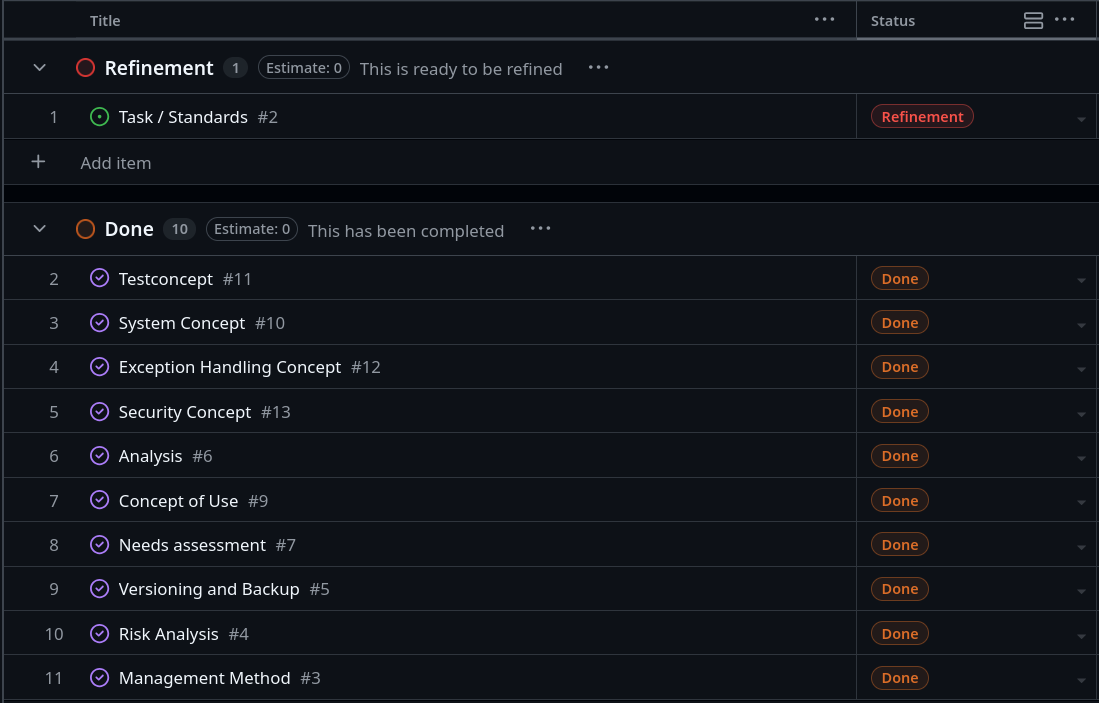
\includegraphics[width=1\textwidth,]{sprint1_backlog.png}}
   \caption{Backlog nach Sprint 1}
\end{figure}

Im Sprint konnten ausgenommen einer User Story alle Stories umgesetzt werden. 
Die User Story "Tasks / Standards" konnte nicht vollständig umgesetzt werden. 
Grund dafür ist das die Abschnitte ``Schutzbedarfsanalyse'', ``Einführung'' und ``Risikoanalyse für Projektrisiken'' in der Dokumentation noch nicht beschrieben wurden. 
Gemäss dem Vorgehen wird die User Story zurück auf die Spalte "Refinement" gesetzt und im kommenden Sprint Planning im neuen Sprint eingeteilt.

\newpage

\section{Sprint Diagramme}

\subsection{Burnup}

\begin{figure}[h]
   \centering
   \fbox{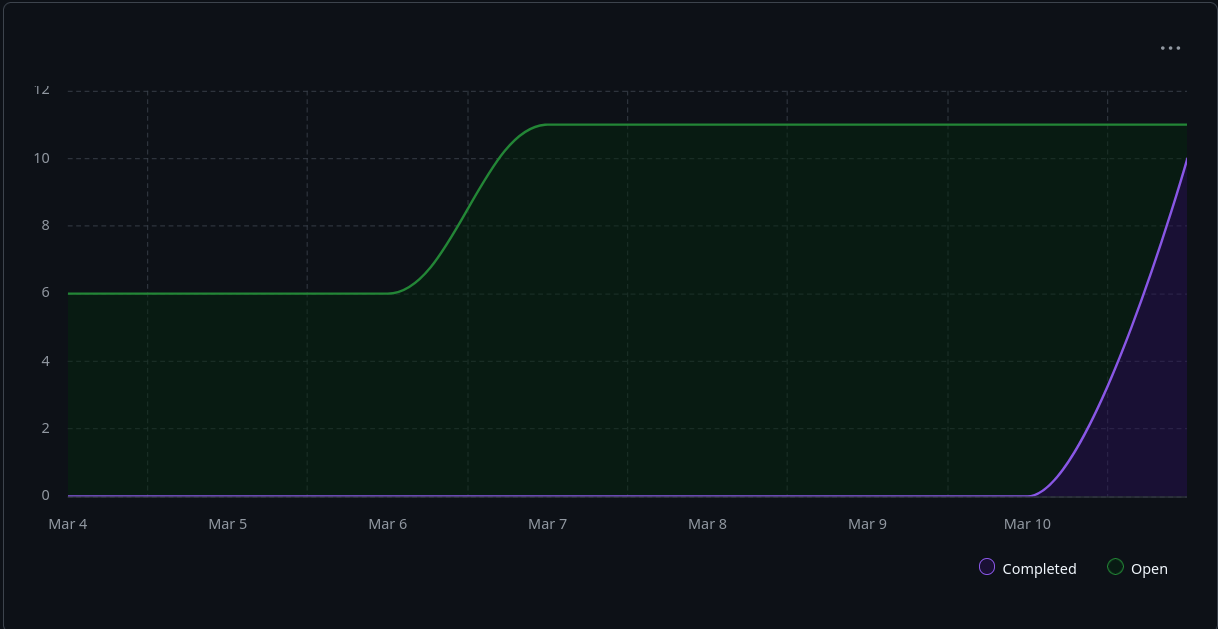
\includegraphics[width=0.8\textwidth,]{sprint1_burnup.png}}
   \caption{Burnup nach Sprint 1}
\end{figure}

Anhand des Burnups sieht man, dass die meisten User Stories bis zum Sprintabschluss abgeschlossen werden konnten.
Die Anzahl der User Stories hat sich am 07.03.2025 erhöht, da die User Story ``Entwurf'' aufgeteilt wurde. Dies geschah auf Anweisung
des Hauptexperten Lorenz Müller.

\subsection{User Story chart}
\begin{figure}[h]
   \centering
   \fbox{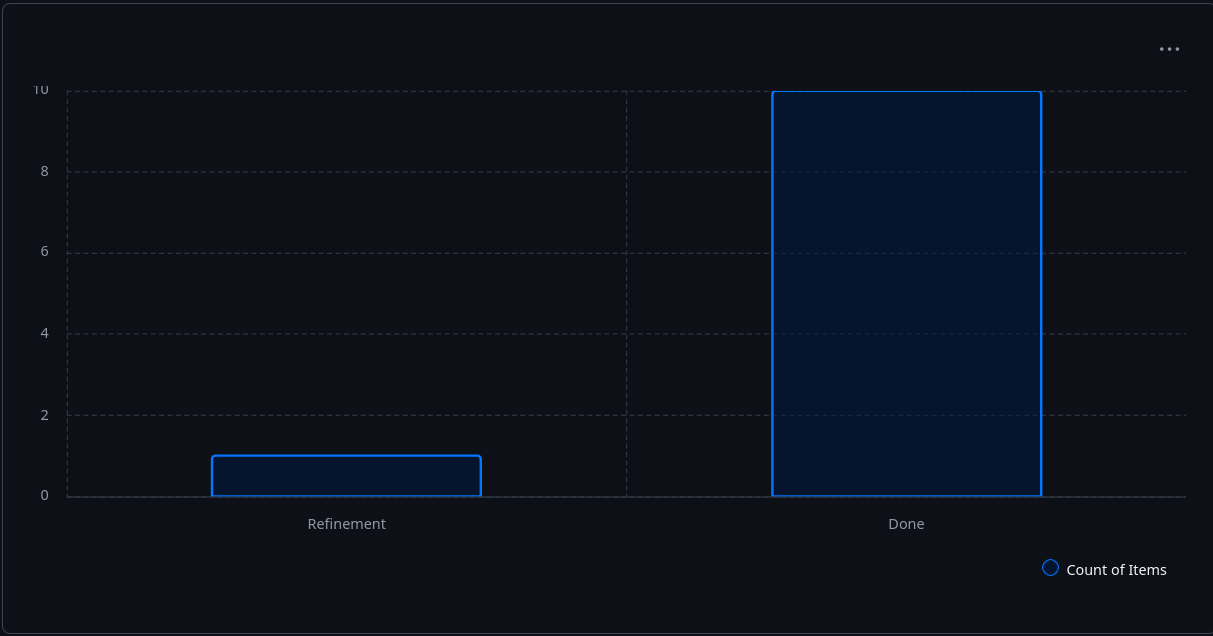
\includegraphics[width=0.8\textwidth,]{sprint1_status_chart.png}}
   \caption{Charts nach Sprint 1}
\end{figure}

Als Fazit werden im obenstehenden Bild die Verteilung der Status aller User Stories im Sprint angezeigt.

\newpage

\chapter{Umsetzung}

\section{Schnittstellen}
Im Entwurf wurde definiert, dass pro Filterkriterium eine Schnittstelle (Endpoint) definiert wird. Während des Implementierens wurde diese Definition geändert.
Grund dafür war die Erkenntniss, dass alle Filterkriterien über die gleichen Schnittstelle geladen werden können. Die Aufgabe der Schnittstelle ist es, 
nur ein Partial zu rendern. Welches Partial gerendert werden muss, wird über einen mitgegebenen Parameter entschieden, welcher den Namen des Filterkriteriums trägt.

Ein Beispiel für einen Request auf diese Schnittstelle: 

\texttt{https:://localhost 3000/people\_filters/tag} 

Der Request kann folgendermassen aufgelöst werden:

\begin{table}[h!]
   \begin{tabular}{|L{0.4\textwidth}|L{0.6\textwidth}|}
       \hline
       \rowcolor{puzzleblue} \multicolumn{2}{|l|}{\color{white}\textbf{Turbo Request}} \\[12pt]
       \hline
        Host & https://localhost:3000 \\
       \hline
       Ressource & /people\_filters \\
       \hline
        Wert des Parameters \texttt{filter\_criterion} & /tag \\
       \hline
       Funktion & Rendert das Tag-Partial \\
     \hline
     \end{tabular}
     \caption{Turbo Request}
\end{table}

Nach dem Muster des oben beschriebenen Requests können sämtliche Partials weiterer Kriterien gerendert werden.
Alle Requests werden dabei von einer Controller-Action behandelt welche durch den Parameter \texttt{filter\_criterion}
entscheidet welches Partial zurückgegeben wird.


\section{Einsatz von KI-Modellen}
\section{Gems}
\subsection{can-can-can}
\subsection{dry-crud}

\chapter{Einführung}

\section{Instruktion}

\section{Unvorhergesehene Änderungen}
\subsection{application.rb}
\subsection{\_list.html.haml}

\chapter{Sprintabschlüsse}

\section{Abschluss Sprint Initialisierung}
\subsection{Backlog}

\section{Abschluss Sprint Umsetzung}
\subsection{Backlog}

\section{Abschluss Sprint Finalisierung}
\subsection{Backlog}


